% !TEX encoding = UTF-8 Unicode
% !TEX root = Simulation.tex

%%%  This is the main driver file.   It is mostly a list of file includes.   Read through and edit as needed.

\documentclass[table]{book}


\usepackage[width=6.5in, height=9.0in, top=1.0in, papersize={8.5in,11in}]{geometry}
\usepackage[pdftex]{graphicx}
\DeclareGraphicsExtensions{.pdf,.png,.jpg}
%\usepackage{draftwatermark}
\usepackage{amsmath}
\usepackage{amsthm}
\usepackage{amssymb}
%\usepackage{txfonts}
\usepackage{textcomp}
%\usepackage{amsthm}
%\usepackage{array}
%\usepackage{datetime}
%\usepackage{anyfontsize}
\usepackage{t1enc}
\usepackage[section,subsection]{extraplaceins}   %%%  \FloatBarrier
\usepackage[all]{xy}
\usepackage{fancyhdr}
\usepackage{hyperref}
\usepackage{verbatim}
\usepackage{algorithm}
\usepackage{algorithmic}
\usepackage{makeidx}
\usepackage{multicol}
\usepackage{multirow}
\usepackage{color}
\usepackage{rotating}
\usepackage{wrapfig}
%\usepackage{tikz}
%\usetikzlibrary{shapes.geometric, arrows}
%\usepackage{tabularx}
\usepackage{xcolor}
%\usepackage{framed}
\usepackage{xspace}
\usepackage{listings}
\usepackage{caption}
\usepackage{subcaption}
\usepackage{enumerate}

\lstset{language=python,frame=ltrb,framesep=5pt,basicstyle=\normalsize,
 keywordstyle=\ttfamily\color{DarkRed},
%morecomment=[n][\textbf]{In\ [}{]\:},
%morecomment=[n][\textbf]{Out\ [}{]\:},
morecomment=[s][\color{blue}]{In\ [}{]\:},
morecomment=[s][\color{red}]{Out[}{]\:},
identifierstyle=\ttfamily\color{DarkBlue}\bfseries,
commentstyle=\color{OliveGreen},
stringstyle=\ttfamily,
showstringspaces=false,tabsize = 3}

\lstdefinelanguage{shell} {
commentstyle = \color{black},
keywordstyle = \color{black},
stringstyle = \color{black},
identifierstyle = \color{black},
morecomment=[s][\color{blue}]{In\ [}{]\:},
morecomment=[s][\color{red}]{Out[}{]\:},
 }

\newtheorem{thrm}{Theorem}
\newtheorem{lem}[thrm]{Lemma}
\newtheorem{cor}[thrm]{Corollary}
\newtheorem{rem}[thrm]{Remark}
\newtheorem{defn}[thrm]{Definition}
\newtheorem{exmpl}[thrm]{Example}

% this gives a little box for the end of a proof:
%
\def\endthrmbox{$\sqsubset \!\!\!\! \sqsupset$}

\newcommand{\dis}{\displaystyle}
 \def      \RR             {{\mathbb R}} 
        \def      \NN             {{\Bbb N}} 
        \def      \QQ             {{\Bbb Q}} 
        \def      \CC             {{\Bbb C}} 
        \def      \ZZ             {{\Bbb Z}} 
 
 
        \def       \a              {{\alpha}} 
        \def       \b              {{\beta}} 
        \def       \d              {{\delta}} 
        \def       \D              {{\Delta}} 
        \def         \e              {{\varepsilon}} 
        \def         \g              {{\gamma}} 
        \def         \G              {{\Gamma}} 
        \def       \l              {{\lambda}} 
        \def       \L              {{\Lambda}} 
        \def        \m               {{\mu}} 
        \def         \n              {{\nabla}} 
        \def       \var          {{\varphi}} 
        \def         \s              {{\sigma}} 
        \def       \Sig          {{\Sigma}} 
        \def       \Om          {{\Omega}} 
 
        \def       \t              {{\tau}} 
        \def         \th             {{\theta}} 
        \def       \O              {{\Omega}} 
        \def       \o              {{\omega}} 
        \def         \z              {{\zeta}} 
       \def        \P             {{\Phi}} 
       \def        \p             {{\phi}} 
        %Other macros 
 
        \def       \iy              {{\infty}} 
        \def         \pa             {{\partial}} 
        \def         \div           {{\rm div}} 
         \def       \na            {{\nabla}} 
 



\newcommand{\pythonlogo}{
\\[-2mm] \begin{picture}(0,0)
\put(-40,-40){\includegraphics[scale=0.25]{./Figures/pythonlogo.png}}
\end{picture}
}

\newcommand{\clogo}{
\\[-2mm] \begin{picture}(0,0)
\put(-30,-30){\includegraphics[scale=0.2]{./Figures/clogo.png}}
\end{picture}
}

\newcommand{\roslogo}{
\\[-2mm] 
\begin{picture}(0,0)
\put(-30,-30){\includegraphics[scale=0.2]{./Figures/roslogo.png}}
\end{picture}
}


%\tikzstyle{master} = [rectangle, draw, text width=6em, text centered, minimum
%height=3em]
%\tikzstyle{node} = [rectangle, draw, text width=6em, text centered, rounded
%corners, minimum height=3em]

\newtheorem{summary}{Summary:}
\newtheorem{example}{Example:}[section]

\definecolor{OliveGreen}{cmyk}{0.64,0,0.95,0.40}
\definecolor{DarkBlue}{cmyk}{0.76,0.76,0,0.20}
\definecolor{DarkRed}{cmyk}{0,1,1,0.45}


\def      \RR             {{\mathbb R}} 
\def      \DS            {\displaystyle} 

\setlength{\oddsidemargin}{0mm} 
\setlength{\evensidemargin}{0mm} 

%\SetWatermarkLightness{0.975}
%\SetWatermarkScale{6}
%\SetWatermarkText{\includegraphics{test.png}}

\pagestyle{fancy}
\renewcommand{\chaptermark}[1]{\markboth{#1}{}}
\renewcommand{\sectionmark}[1]{\markright{\thesection\ #1}}
\fancyhf{}
\fancyhead[LE,RO]{\bfseries\thepage}
\fancyhead[LO]{\bfseries\rightmark}
\fancyhead[RE]{\bfseries\leftmark}
\renewcommand{\headrulewidth}{0.5pt}
\renewcommand{\footrulewidth}{0pt}
\addtolength{\headheight}{0.5pt}
\setlength{\footskip}{0in}
\renewcommand{\footruleskip}{0pt}
\fancypagestyle{plain}{%
\fancyhead{}
\renewcommand{\headrulewidth}{0pt}
}


\definecolor{color02}{rgb}{0.18,0.35,0.59}
\definecolor{color03}{rgb}{0.44,0.59,0.82}
\definecolor{color06}{rgb}{0.35,0.35,0.35}


\definecolor{MSBlue}{rgb}{.204,.353,.541}
\definecolor{MSLightBlue}{rgb}{.31,.506,.741}
\definecolor{MSBlue1}{rgb}{0.18,0.35,0.59}
\definecolor{MSBlue2}{rgb}{0.44,0.59,0.82}
\definecolor{MSBlue3}{rgb}{0.35,0.35,0.35}

\usepackage{titlesec}
\titleformat{\chapter}[display]
%{\normalfont\bfseries\color{MSBlue1}}    %\normalfont\bfseries\filcenter}
{\normalfont\bfseries}    %\normalfont\bfseries\filcenter}
{\LARGE\thechapter}
{1ex}
{\titlerule[2pt]
\vspace{2ex}%
\LARGE}
[\vspace{1ex}%
{\titlerule[2pt]}]



\date{\today}

 % This sets the format.

\graphicspath{ {images/} }

\newcommand{\includecode}[1]{\lstinputlisting[caption={\detokenize{#1}}, label={\detokenize{#1}}]{\detokenize{code/#1}}}

\lstset{language=Python, basicstyle=\ttfamily}

% Add your title page contents here 
\title{{ \rule{\linewidth}{0.5mm}}\\[2mm] {\huge \bfseries  Simulation }\\[-1mm] {\rule{\linewidth}{0.5mm}} \\  \vfill
{\LARGE \bfseries  Natural Computing Homework }\vfill}
\author{Stephanie Athow \and  Chris Smith}
\date{\today}


\begin{document}

\frontmatter

% Comment out items you don't need

\addcontentsline{toc}{chapter}{Title}
\maketitle
\tableofcontents
\addcontentsline{toc}{chapter}{Contents}
\listoffigures
\addcontentsline{toc}{chapter}{List of Figures}
\listoftables
\addcontentsline{toc}{chapter}{List of Tables}
\listofalgorithms
\addcontentsline{toc}{chapter}{List of Algorithms}

\chapter{Document Preparation and Updates}
% !TEX root = Simulation.tex



Current Version [X.X.X]
\vspace*{5mm}

{\color{MSBlue3}
\noindent
\textit{Prepared By:}\\
\textit{Team Member \#1}\\
\textit{Team Member \#2}\\
\textit{Team Member \#3}
}

\vfill
\noindent
{\color{color02} \textit{\textbf{Revision History}}}\\
\begin{tabular}{|>{\raggedright}p{1.5cm}|>{\raggedright}p{3cm}|>{\raggedright}p{1.5cm}|>{\raggedright}p{9cm}|}
\hline
\textit{\textbf{Date}} &  \textit{\textbf{Author}} & \textit{\textbf{Version}} & \textit{\textbf{Comments}}\tabularnewline
\hline
 \textit{\textbf{2/2/15}} & \textit{Team Member \#1} & \textit{1.0.0} & \textit{Initial version}\tabularnewline
\hline
\textit{\textbf{3/4/15}} & \textit{Team Member \#3} & \textit{1.1.0} & \textit{Edited version}\tabularnewline
\hline
 &  &  & \tabularnewline
 \hline
 &  &  & \tabularnewline
\hline
 &  &  & \tabularnewline
\hline
 &  &  & \tabularnewline
\hline
 &  &  & \tabularnewline
\hline
\end{tabular}
\vfill


 
 % Core content to follow ...
 
\mainmatter

%%  Add to the following chapters
% you may also need additional chapters ...

% !TEX root = Simulation.tex

\chapter{Fractals - Text Chapter 7}

\section{Problem 10}
\textbf{ Implement a bracketed OL-system and reproduce all plant-like structures of Figure 7.24 [of the book]. Change some derivation rules and see what happens. Make your own portfolio with, at least, ten plants. }

\begin{figure}[tbh]
\begin{center}
	\begin{subfigure}[tbh]{0.3\textwidth}
	\begin{center}
	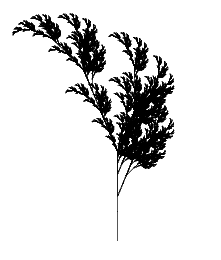
\includegraphics[width=\textwidth]{ferns/plant1.png}
	\caption{Plant 1}
	\end{center}
	\end{subfigure}
\hfill
	\begin{subfigure}[tbh]{0.3\textwidth}
	\begin{center}
	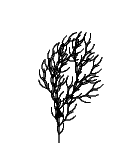
\includegraphics[width=\textwidth]{ferns/plant2.png}
	\caption{Plant 2}
	\end{center}
	\end{subfigure}
\hfill
	\begin{subfigure}[tbh]{0.3\textwidth}
	\begin{center}
	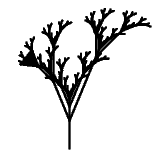
\includegraphics[width=\textwidth]{ferns/plant3.png}
	\caption{Plant 3}
	\end{center}
	\end{subfigure}
\hfill
	\begin{subfigure}[tbh]{0.3\textwidth}
	\begin{center}
	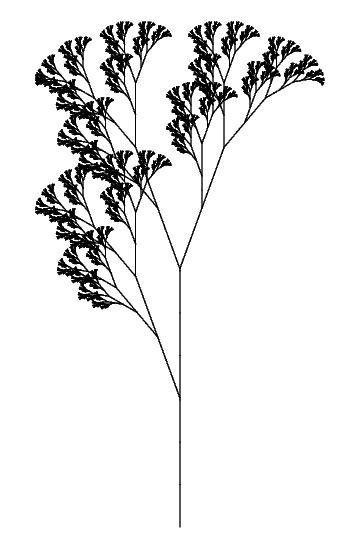
\includegraphics[width=\textwidth]{ferns/plant4.png}
	\caption{Plant 4}
	\end{center}
	\end{subfigure}
\hfill
	\begin{subfigure}[tbh]{0.3\textwidth}
	\begin{center}
	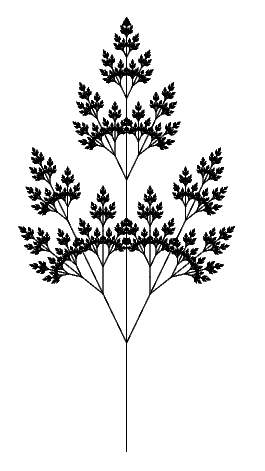
\includegraphics[width=\textwidth]{ferns/plant5.png}
	\caption{Plant 5}
	\end{center}
	\end{subfigure}
\hfill
	\begin{subfigure}[tbh]{0.3\textwidth}
	\begin{center}
	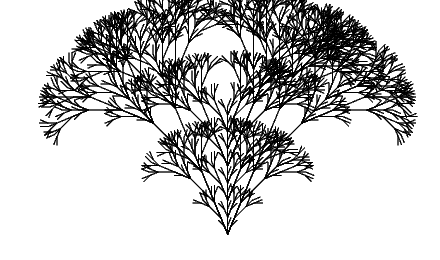
\includegraphics[width=\textwidth]{ferns/plant6.png}
	\caption{Plant 6}
	\end{center}
	\end{subfigure}
\hfill
\end{center}
\caption{ Plants from "Fundamentals of Natural Computing}
\end{figure} \label{bookPlants}

\begin{figure}[tbh]
\begin{center}
	\begin{subfigure}[tbh]{0.23\textwidth}
	\begin{center}
	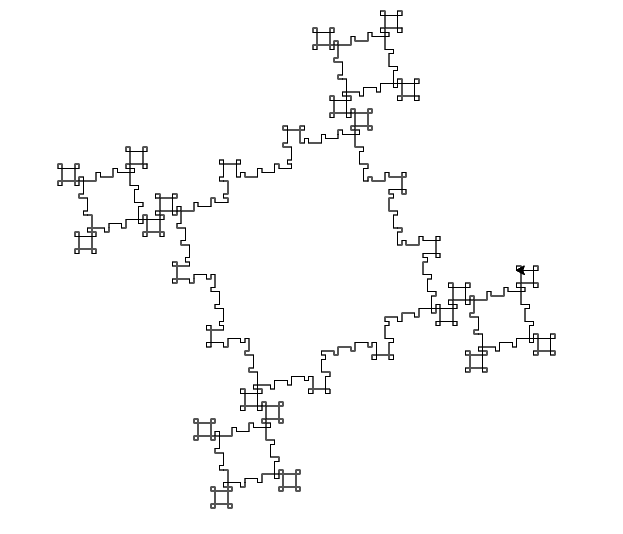
\includegraphics[width=\textwidth]{ferns/my-plant1.png}
	\caption{My Plant 1}
	\end{center}
	\end{subfigure}
\hfill
	\begin{subfigure}[tbh]{0.23\textwidth}
	\begin{center}
	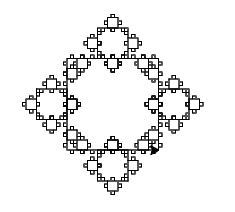
\includegraphics[width=\textwidth]{ferns/my-plant2.png}
	\caption{My Plant 2}
	\end{center}
	\end{subfigure}
\hfill
	\begin{subfigure}[tbh]{0.23\textwidth}
	\begin{center}
	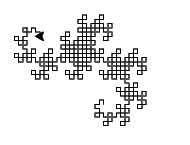
\includegraphics[width=\textwidth]{ferns/my-plant3.png}
	\caption{My Plant 3}
	\end{center}
	\end{subfigure}
\hfill
	\begin{subfigure}[tbh]{0.23\textwidth}
	\begin{center}
	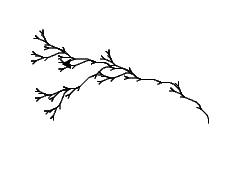
\includegraphics[width=\textwidth]{ferns/my-plant4.png}
	\caption{My Plant 4}
	\end{center}
	\end{subfigure}
\hfill
	\begin{subfigure}[tbh]{0.23\textwidth}
	\begin{center}
	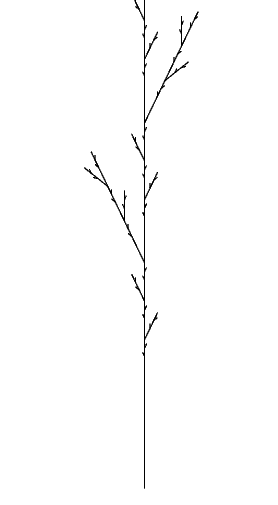
\includegraphics[width=\textwidth]{ferns/my-plant5.png}
	\caption{My Plant 5}
	\end{center}
	\end{subfigure}
\hfill
	\begin{subfigure}[tbh]{0.23\textwidth}
	\begin{center}
	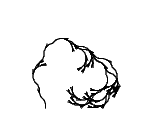
\includegraphics[width=\textwidth]{ferns/my-plant6.png}
	\caption{My Plant 6}
	\end{center}
	\end{subfigure}
\hfill
	\begin{subfigure}[tbh]{0.23\textwidth}
	\begin{center}
	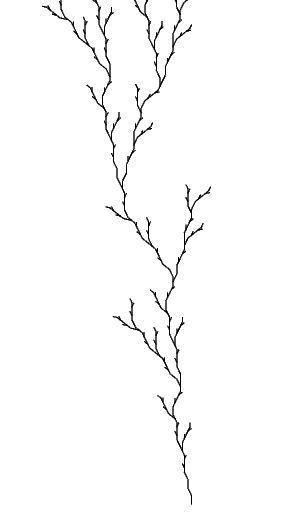
\includegraphics[width=\textwidth]{ferns/my-plant7.png}
	\caption{My Plant 7}
	\end{center}
	\end{subfigure}
\hfill
	\begin{subfigure}[tbh]{0.23\textwidth}
	\begin{center}
	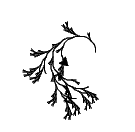
\includegraphics[width=\textwidth]{ferns/my-plant8.png}
	\caption{My Plant 8}
	\end{center}
	\end{subfigure}
\hfill
	\begin{subfigure}[tbh]{0.23\textwidth}
	\begin{center}
	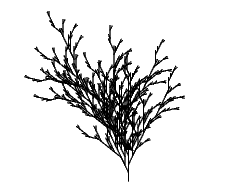
\includegraphics[width=\textwidth]{ferns/my-plant9.png}
	\caption{My Plant 9}
	\end{center}
	\end{subfigure}
\hfill
	\begin{subfigure}[tbh]{0.23\textwidth}
	\begin{center}
	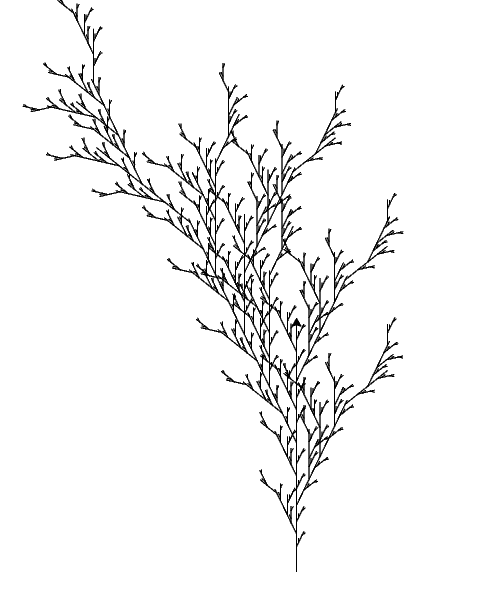
\includegraphics[width=\textwidth]{ferns/my-plant10.png}
	\caption{My Plant 10}
	\end{center}
	\end{subfigure}
\hfill
\end{center}
\caption{ Plants from "Fundamentals of Natural Computing}
\end{figure} \label{myPlants}

\section{Problem 15}
\textbf{ Implement a RIFS to generate all the fractals whose codes are presented in Table: ~\ref{table:RIFS} } \\
\newline
RIFS is an acronym for Random Iterated Function System (RIFS). An iterated function system (IFS) recursively applies a set of affine transformations to each point in a point list. Generally, the affine transformations are a contractive mapping.  Unless you are zooming in, there is a depth at which the points are very dense and not all of them need to be mapped. This is where the RIFS comes into play. Each point in the point list has one of the functions of the set applied to it. The resolution is still good and the program runs much faster because there are few computations done. 

The codes (functions) given in ~\ref{table:RIFS} are defined such that \textit{w} is the function number, \textit{a, b, c, d} are scaling factors, \textit{e, f} are offset values and \textit{p} is the probability the function will be selected. These values are used in the equation for affine transformation ~\ref{affine_transformation}. The Sierpinski Gasket and Square fractals must have an initial point list to perform the transformations. The Barnsley Fern and Tree need only a single point to perform the transformations. Figure ~\ref{fractals} shows the Sierpinski Gasket, Square, Bransley Fern and Tree generated using the RIFS codes. 

\begin{equation}
w(x_1 , x_2) = ( a x_1 + b x_2 + e, c x_1 + d x_2 + f )
\end{equation} \label{affine_transformation}

\begin{figure}[tbh]
\begin{center}
	\begin{subfigure}[tbh]{0.475\textwidth}
	\begin{center}
	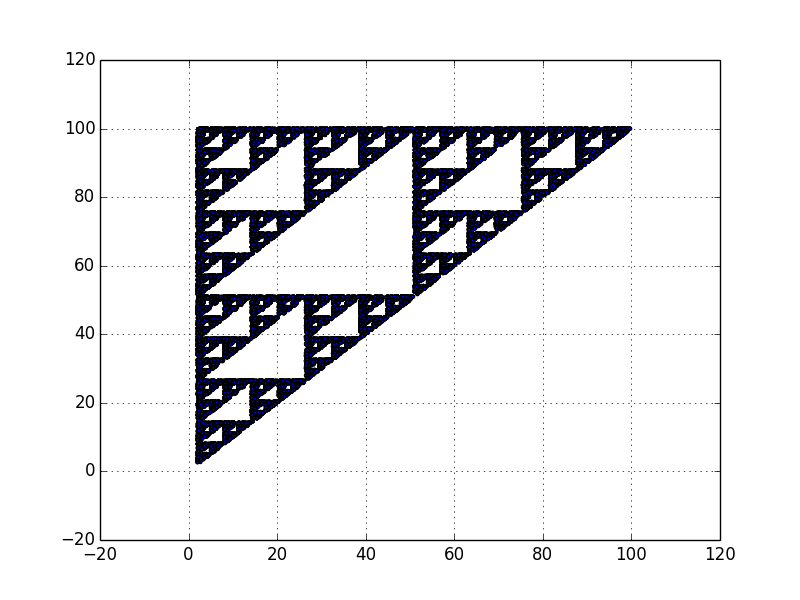
\includegraphics[width=\textwidth]{fractals/SierpinskiGasket.png}
	\caption{ Sierpinski Gasket }
	\end{center}
	\end{subfigure}
\hfill
	\begin{subfigure}[tbh]{0.475\textwidth}
	\begin{center}
	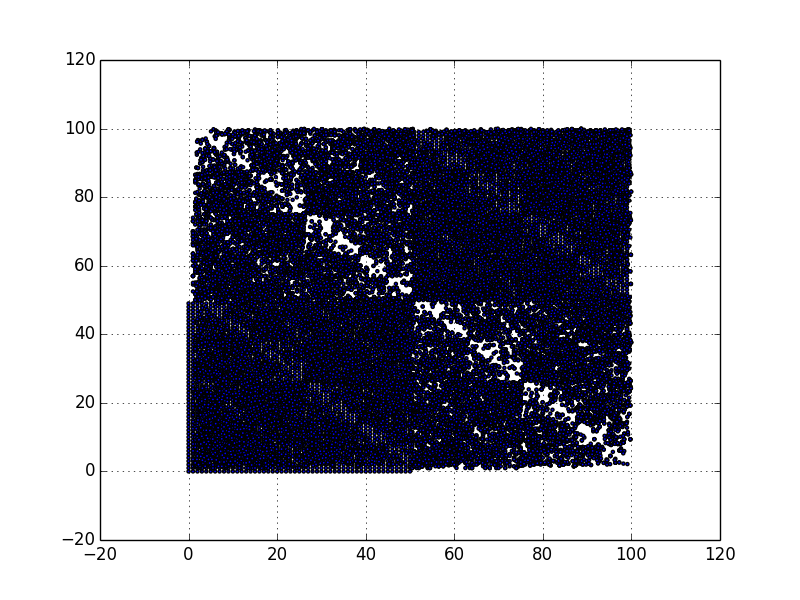
\includegraphics[width=\textwidth]{fractals/Square.png}
	\caption{ Square }
	\end{center}
	\end{subfigure}
\hfill
	\begin{subfigure}[tbh]{0.475\textwidth}
	\begin{center}
	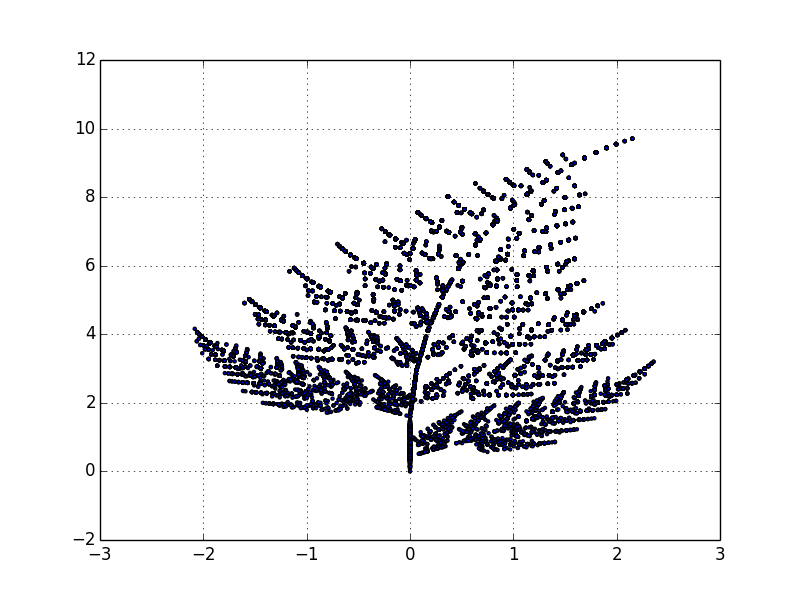
\includegraphics[width=\textwidth]{fractals/BarnsleyFern.png}
	\caption{ Barnsley Fern }
	\end{center}
	\end{subfigure}
\hfill
	\begin{subfigure}[tbh]{0.475\textwidth}
	\begin{center}
	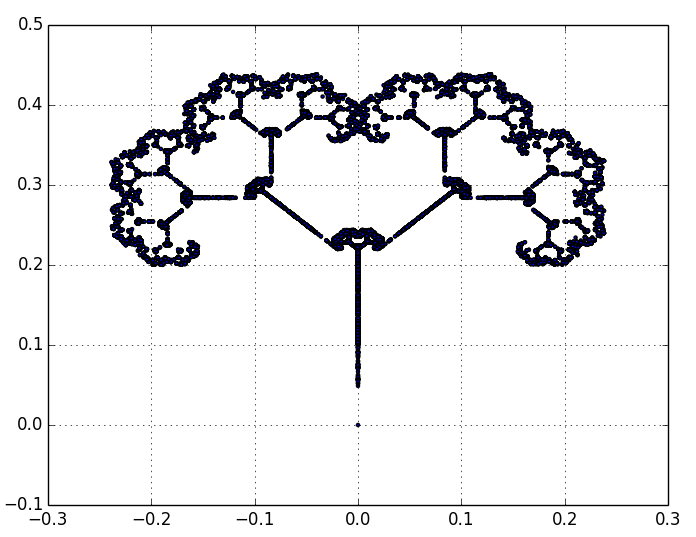
\includegraphics[width=\textwidth]{fractals/Tree.png}
	\caption{ Tree }
	\end{center}
	\end{subfigure}
\hfill

\end{center}
\caption{Plots of Various Fractals \label{fractals} }
\end{figure}

\begin{table}[ht]
\caption{RIFS codes to generate fractals} 
	\subcaption{Sierpinski Gasket}
	\centering 
	\begin{tabular}{c c c c c c c c} 
	\hline\hline 
	w & a & b & c & d & e & f & p\\ [0.5ex] 
	\hline 
	1 & 0.5 & 0 & 0 & 0.5 & 1 & 1 & 0.33 \\
	2 & 0.5 & 0 & 0 & 0.5 & 1 & 50 & 0.33\\
	3 & 0.5 & 0 & 0 & 0.5 & 50 & 50 & 0.34 \\
	\hline 
\end{tabular}
\bigskip
	\subcaption{ Square }
	\centering 
	\begin{tabular}{c c c c c c c c} 
	\hline\hline 
	w & a & b & c & d & e & f & p\\ [0.5ex] 
	\hline 
	1 & 0.5 & 0 & 0 & 0.5 & 1 & 1 & 0.25\\
	2 & 0.5 & 0 & 0 & 0.5 & 50 & 1 & 0.25\\
	3 & 0.5 & 0 & 0 & 0.5 & 1 & 50 & 0.25\\
	4 & 0.5 & 0 & 0 & 0.5 & 50 & 50 & 0.25\\
	\hline 
\end{tabular}
\bigskip
	\subcaption{ Barnsley Fern }
	\centering 
	\begin{tabular}{c c c c c c c c} 
	\hline\hline 
	w & a & b & c & d & e & f & p\\ [0.5ex] 
	\hline 
	1 & 0 & 0 & 0 & 0.16 & 0 & 0 & 0.01 \\
	2 & 0.85 & 0.04 & -0.04 & 0.85 & 0 & 1.6 & 0.85\\
	3 & 0.2 & -0.26 & 0.23 & 0.22 & 0 & 1.6 & 0.07 \\
	4 & -0.15 & 0.28 & 0.26 & 0.24 & 0 & 0.44 & 0.07 \\
	\hline 
\end{tabular}
\bigskip
	\subcaption{ Tree }
	\centering 
	\begin{tabular}{c c c c c c c c} 
	\hline\hline 
	w & a & b & c & d & e & f & p\\ [0.5ex] 
	\hline 
	1 & 0 & 0 & 0 & 0.5 & 0 & 0 & 0.05 \\
	2 & 0.42 & -0.42 & 0.42 & 0.42 & 0 & 0.2 & 0.40\\
	3 & 0.42 & 0.42 & -0.42 & 0.42 & 0 & 0.2 & 0.40\\
	4 & 0.1 & 0 & 0 & 0.1 & 0 & 0.2 & 0.15 \\
	\hline 
\end{tabular}
\end{table} \label{table:RIFS}


\section{ Problem 21 }
\textbf{ Implement the random midpoint displacement algorithm in 3D and generate some fractal landscapes. Study the influence of \textit{H} on the landscapes generated. } \\
\newline

In 2D, the random midpoint displacement starts with a line, determines the midpoint and randomly perturbs it using equations ~\ref{midpointDisplacement} and ~\ref{roughness}. In equation ~\ref{roughness}, $\Delta(i)$ stores the value for depth $i$, $\sigma$ is the standard deviation of the Gaussian distribution, $H$ is the `roughness factor'. $H$ is always $ 0 < H < 1$. The closer to 0, the more rough the surface will be. The closer to 1, the more smooth the surface will be.  In equation ~\ref{midpointDisplacement} $x_1$ is the new value for the midpoint, $x_0$ is the left end point, $x_2$ is the right end point, $\Delta(t)$ is  from equation ~\ref{roughness}, $t$ is the recursion depth and $rand$ is a random number. Now, there are two line segments and the midpoint of each line segment is perturbed. This method is recursively applied while decreasing the perturbation amount for each depth. 

\begin{equation}
x_1 = 0.5 ( x_0 + x_2 ) + \Delta(t)  rand
\end{equation} \label{midpointDisplacement}

\begin{equation}
\Delta(i) = \sigma (H)^{(i+1)/2)}
\end{equation} \label{roughness}

The random midpoint displacement for 3D starts with a 2D box. The box is subdivided using the midpoints of the edges, so one box becomes four boxes, four boxes becomes sixteen, ect. The intersections of the midpoint lines becomes the perturbation points. They are perturbed in the same manner as the 2D method except the average is the average of the four surrounding points. Figure ~\ref{surfaces} shows some surfaces with varying $H$ values.


\begin{figure}[tbh]
\begin{center}
	\begin{subfigure}[tbh]{0.475\textwidth}
	\begin{center}
	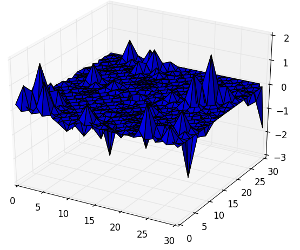
\includegraphics[width=\textwidth]{fractals/brownianSurface_s1-5_H0-2.png}
	\caption{ $\sigma = 1.5$, $H = 0.2$ }
	\end{center}
	\end{subfigure}
\hfill
	\begin{subfigure}[tbh]{0.475\textwidth}
	\begin{center}
	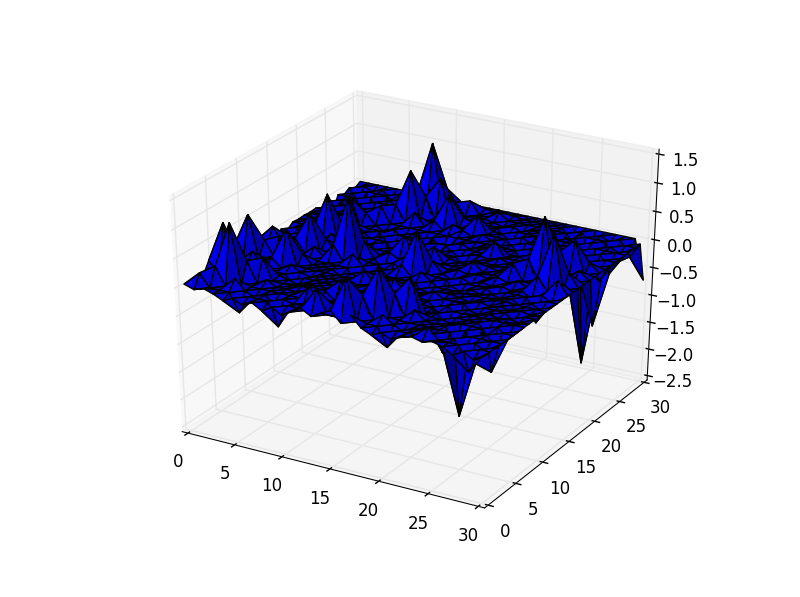
\includegraphics[width=\textwidth]{fractals/brownianSurface_s1-5_H0-5.png}
	\caption{$\sigma = 1.5$, $H = 0.5$}
	\end{center}
	\end{subfigure}
\hfill
	\begin{subfigure}[tbh]{0.475\textwidth}
	\begin{center}
	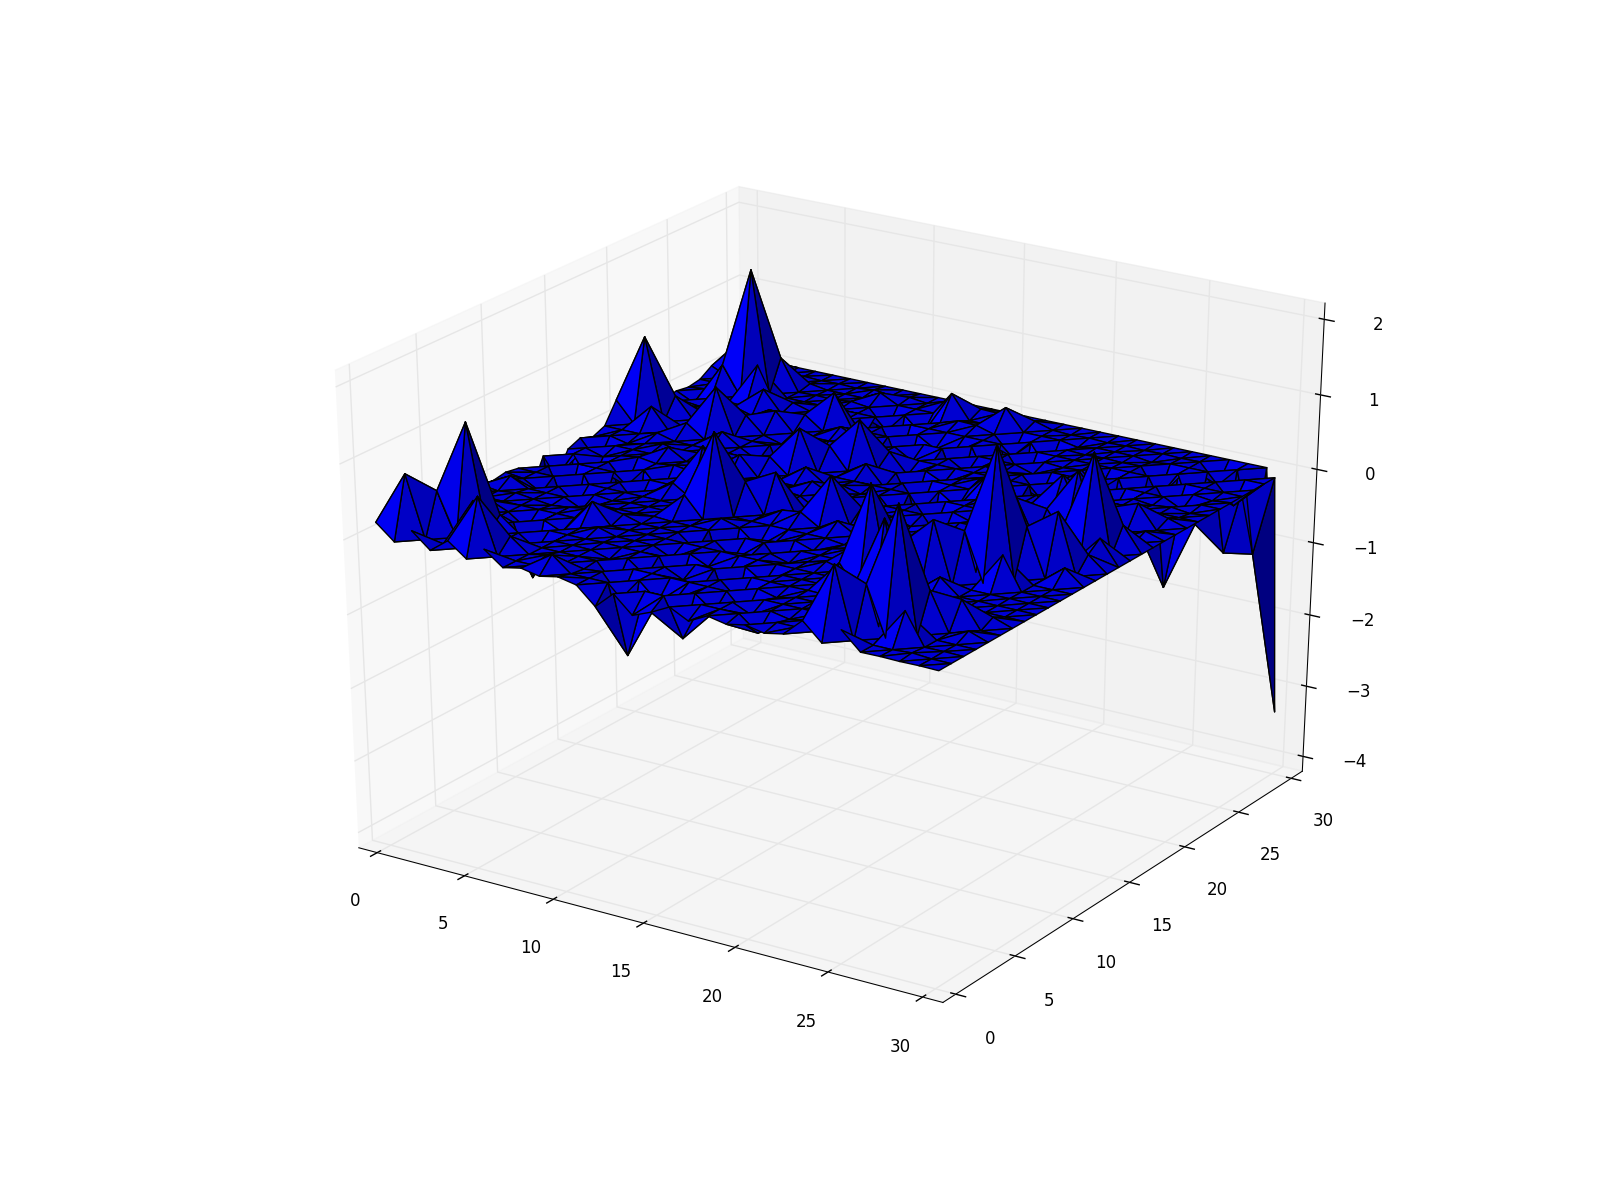
\includegraphics[width=\textwidth]{fractals/brownianSurface_s1-5_H0-75.png}
	\caption{ $\sigma = 1.5$, $H = 0.75$ }
	\end{center}
	\end{subfigure}
\hfill
	\begin{subfigure}[tbh]{0.475\textwidth}
	\begin{center}
	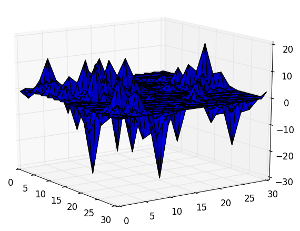
\includegraphics[width=\textwidth]{fractals/brownianSurface_s5_H0-75.png}
	\caption{ $\sigma = 5$, $H = 0.75$ }
	\end{center}
	\end{subfigure}
\hfill

\end{center}
\caption{Brownian Surfaces with Varying $\sigma$'s and $H$'s \label{surfaces} }
\end{figure}

t%!TEX root = Simulation.tex

\chapter{Cellular Automata - Chapter 7}

\section{Problem: Slides 1}
\textbf{ Modify the heat flow example to deal with insulated conditions on the top and bottom boundary. Insulation means zero flux or u[N][j] = u[N-1][j]. This implies that instead of a fixed valued ghost points on the top and bottom, you modify the CA rule using the previous relation. }\\
\newline
Cellular automata can be used to study some types of dynamics. In this case, a box with insulated top and bottom walls, and a parabolic heat source on the right wall is presented. The insulated conditions means that the top and bottom boundaries are equal to the grid square below and above them. Using the four neighbors rule, the simplified equation ~\ref{heatDiscrete} is applied to $N-2$ by $N-2$ squares.

Figure ~\ref{heatFlow} shows a grid of 25 x 25 on the left and a grid of 100 x 100 on the right. With the finer grid, a much smoother gradient appears than when using the courser grid. Additionally, the left grid spreads nearly to the left edge before it cools where as the right grid cools approximently halfway across the grid. 

\begin{figure}[tbh]
\begin{center}
	\begin{subfigure}[tbh]{0.47\textwidth}
	\begin{center}
	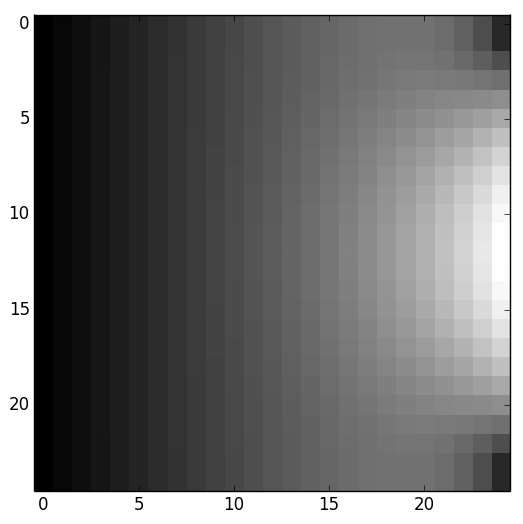
\includegraphics[width=\textwidth]{heatflow/25x25grid10temp.png}
	\caption{ 25 x 25 grid, Temperature = 10 }
	\end{center}
	\end{subfigure}
\hfill
	\begin{subfigure}[tbh]{0.47\textwidth}
	\begin{center}
	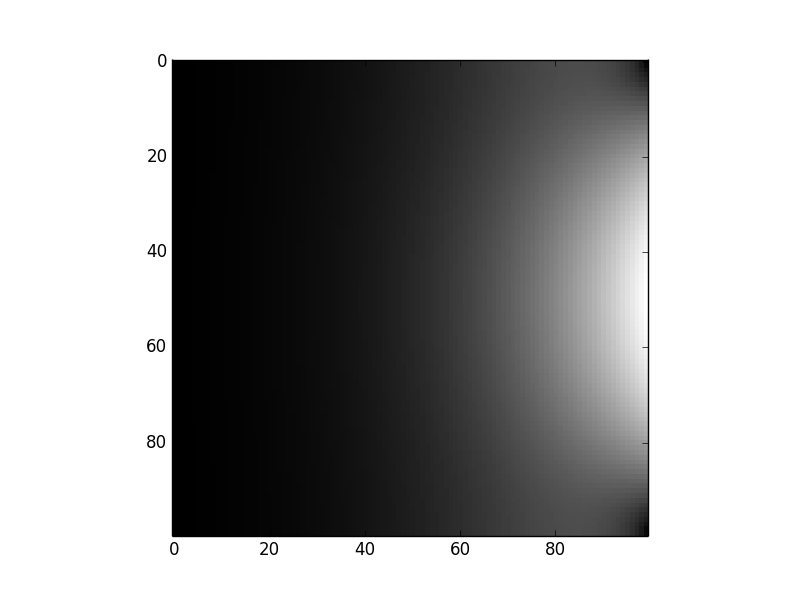
\includegraphics[width=\textwidth]{heatflow/100x100grid10temp.png}
	\caption{ 100 x 100 grid, Temperature = 10 }
	\end{center}
	\end{subfigure}
\hfill
\caption{ Example Heat Flow Grids } \label{heatFlow}
\end{center}
\end{figure}

\begin{equation}
c_{i,j}(t+1) = ( c_{i-1,j}(t) + c_{i+1,j}(t) + c_{i,j-1}(t) + c_{i,j+1}(t)) / 4
\end{equation} \label{heatDiscrete}

\section{Problem: Slides 2}
\textbf{ Reproduce patterns theta, lambda, mu, alpha in the Gray-Scott Model (CA). You don't need to follow their color scheme. } \\
\newline
The Gray-Scott model is used to model pattern formation. The general idea is there's a steady-state grid of some chemical, let's call it $u$. Then, it is perturbed with noise and in the middle with a second chemical, call this one $v$, which reacts with the first chemical. With time, the chemicals reach a steady-state again and a pattern emerges. In equations ~\ref{eqn-grayScott1} and ~\ref{eqn-grayScott2}, $u$ and $v$ are the chemicals reacting, $F$ and $k$ are tuneable parameters which will produce different patterns. Typical values are $ 0.00 < F < 0.08 $ and $ 0.03 < k < 0.07 $ and Figure ~\ref{grayScott-chart} shows values that produce various named patterns.\\

  Using Dr. McGough's code provided on his class website (http://www.mcs.sdsmt.edu/jmcgough/csc492/) and changing the $F$ and $k$ parameters, the images in Figure ~\ref{grayscott-produced} were created. Patterns $\alpha$, $\theta$, and  $\lambda$ are very similar to the examples given in the lecture slides. However, pattern $\mu$ does not compare well to the example. Potential sources of error are gize size, grid granuality or an incorrectly estimated value.

\begin{equation}
\frac{ \partial u}{ \partial t } = d_1  \Delta u - uv^2 + F(1-u)
\end{equation} \label{eqn-grayScott1}

\begin{equation}
\frac{ \partial v}{ \partial t } = d_2 \Delta v + uv^2 - (F+k)v
\end{equation} \label{eqn-grayScott2}

\begin{figure}[tbh]
\begin{center}
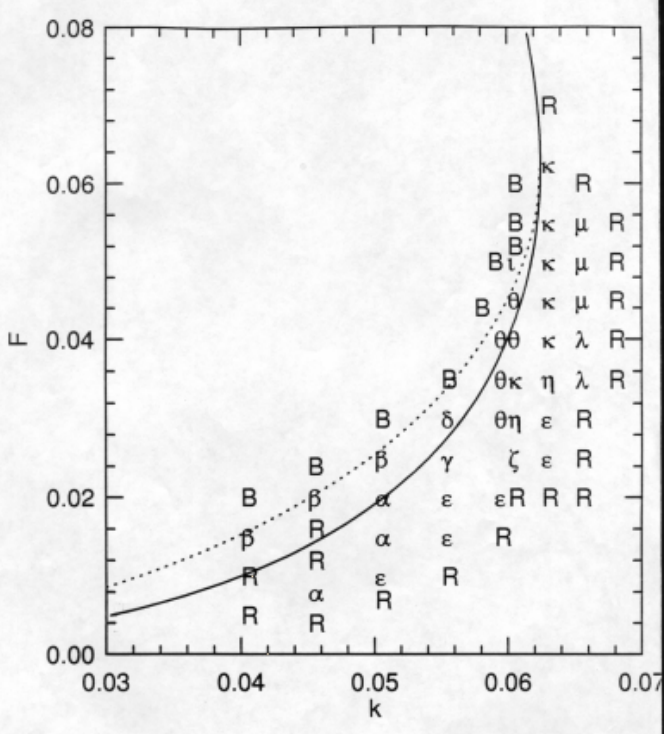
\includegraphics[width=0.47\textwidth]{grayscott/grayscott-chart.png}
\caption{ Gray-Scott Chart }
\end{center}
\end{figure}\label{grayScott-chart}

\begin{figure}[tbh]
\begin{center}
	\begin{subfigure}[tbh]{0.475\textwidth}
	\begin{center}
	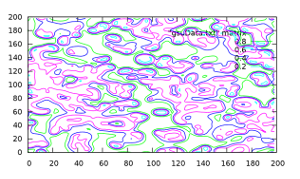
\includegraphics[width=\textwidth]{grayscott/grayscott-alpha.png}
	\caption{ pattern $\alpha$ }
	\end{center}
	\end{subfigure}
\hfill
	\begin{subfigure}[tbh]{0.475\textwidth}
	\begin{center}
	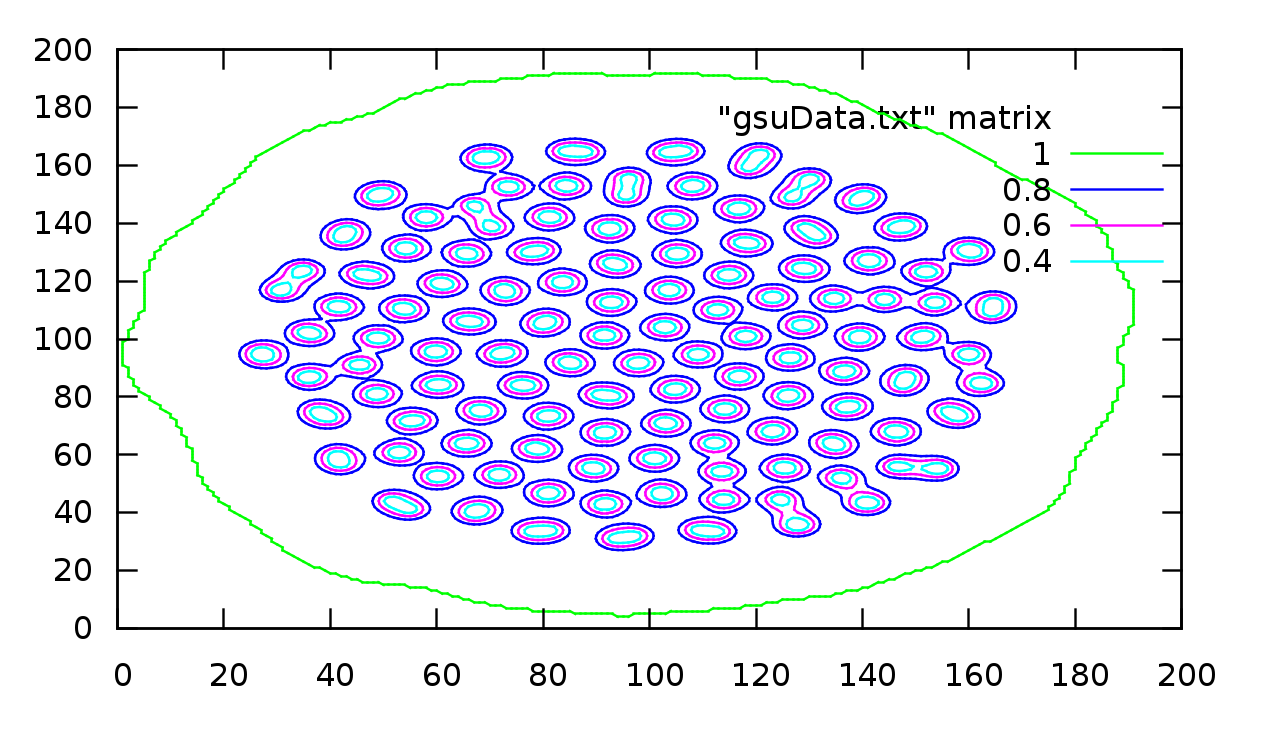
\includegraphics[width=\textwidth]{grayscott/grayscott-lambda.png}
	\caption{ pattern $\lambda$ }
	\end{center}
	\end{subfigure}
\hfill
	\begin{subfigure}[tbh]{0.475\textwidth}
	\begin{center}
	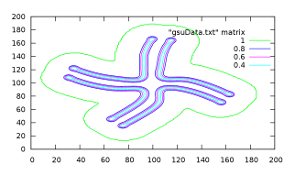
\includegraphics[width=\textwidth]{grayscott/grayscott-mu.png}
	\caption{ pattern $\mu$ }
	\end{center}
	\end{subfigure}
\hfill
	\begin{subfigure}[tbh]{0.475\textwidth}
	\begin{center}
	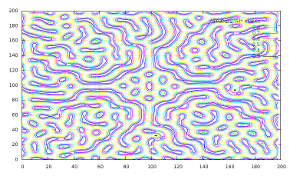
\includegraphics[width=\textwidth]{grayscott/grayscott-theta.png}
	\caption{ pattern $\theta$ }
	\end{center}
	\end{subfigure}
\hfill

\end{center}
\caption{Various Gray-Scott Patterns \label{grayscott-produced} }
\end{figure}
% !TEX root = Simulation.tex

\chapter{ALife - Text Chapter 8}

\section{ Problem 3 }
\textbf{ Choose one of the sample project of StarLogo and solve its exploration tasks (http://education.mit.edu/starlogo/projects.html). Write a brief report with the results obtained including any theoretical background knowledge that may eventually be necessary to perform the explorations. } \\
\newline
\textbf{Exploration questions:}\\
\textbf{Modify the program so that the creatures aggregate into a single large cluster more quickly.}\\
\textbf{How do the results change if there is more (or less) randomness in the creature's motion?}\\
\textbf{What "critical number" of creatures is needed for clusters to form? How does the critical number change if you change the evaporation or diffusion rate?}\\
\newline

By reducing the randomness, usually around 10 - 30, the creatures aggregated into a large cluster fairly quickly - a few minutes at most. Decreasing the rate of evaporation also decreased the aggregation time for the creatures since it would help 'catch' stray creatures. However, at the low random rates, such as in Figures ~\ref{mold1010}, ~\ref{mold2020} and ~\ref{mold3030} a creature or two would occasionally break free from the group and that would cause several others to also break free and form small clusters. This is well illustrated in Figure ~\ref{mold3030} where the middle images shows a fairly cohesive large cluster and the right image is after some groups broke free. 

Interestingly enough, with random values of 70, the creatures quickly formed small groups but were very slow to form two large groups, illustrated in Figure ~\ref{mold7070}. The two large groups would exchange members every now and then but never converged into a large group.

Around 500 - 600 hundred creatures while a pheromone evaporation of 2-4 was the 'critical number' for quick cluster formation. Too few creatures and they had a hard time finding each other. Too many creatures and there was too much pheromone deposited to form a big cluster. 

% 1010
\begin{figure}[tbh]
\begin{center}
	\begin{subfigure}[tbh]{0.30\textwidth}
	\begin{center}
	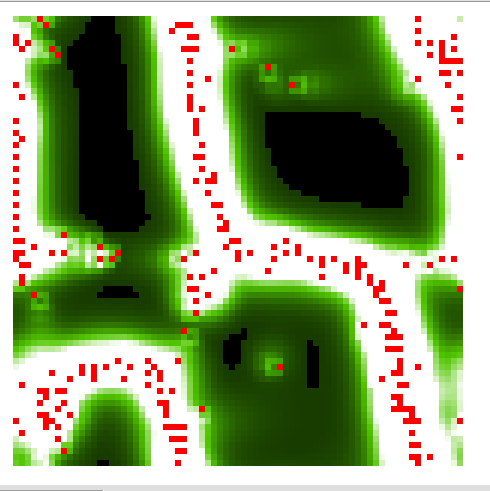
\includegraphics[width=\textwidth]{slimemold/mold10104-1.png}
	\end{center}
	\end{subfigure}
\hfill
	\begin{subfigure}[tbh]{0.30\textwidth}
	\begin{center}
	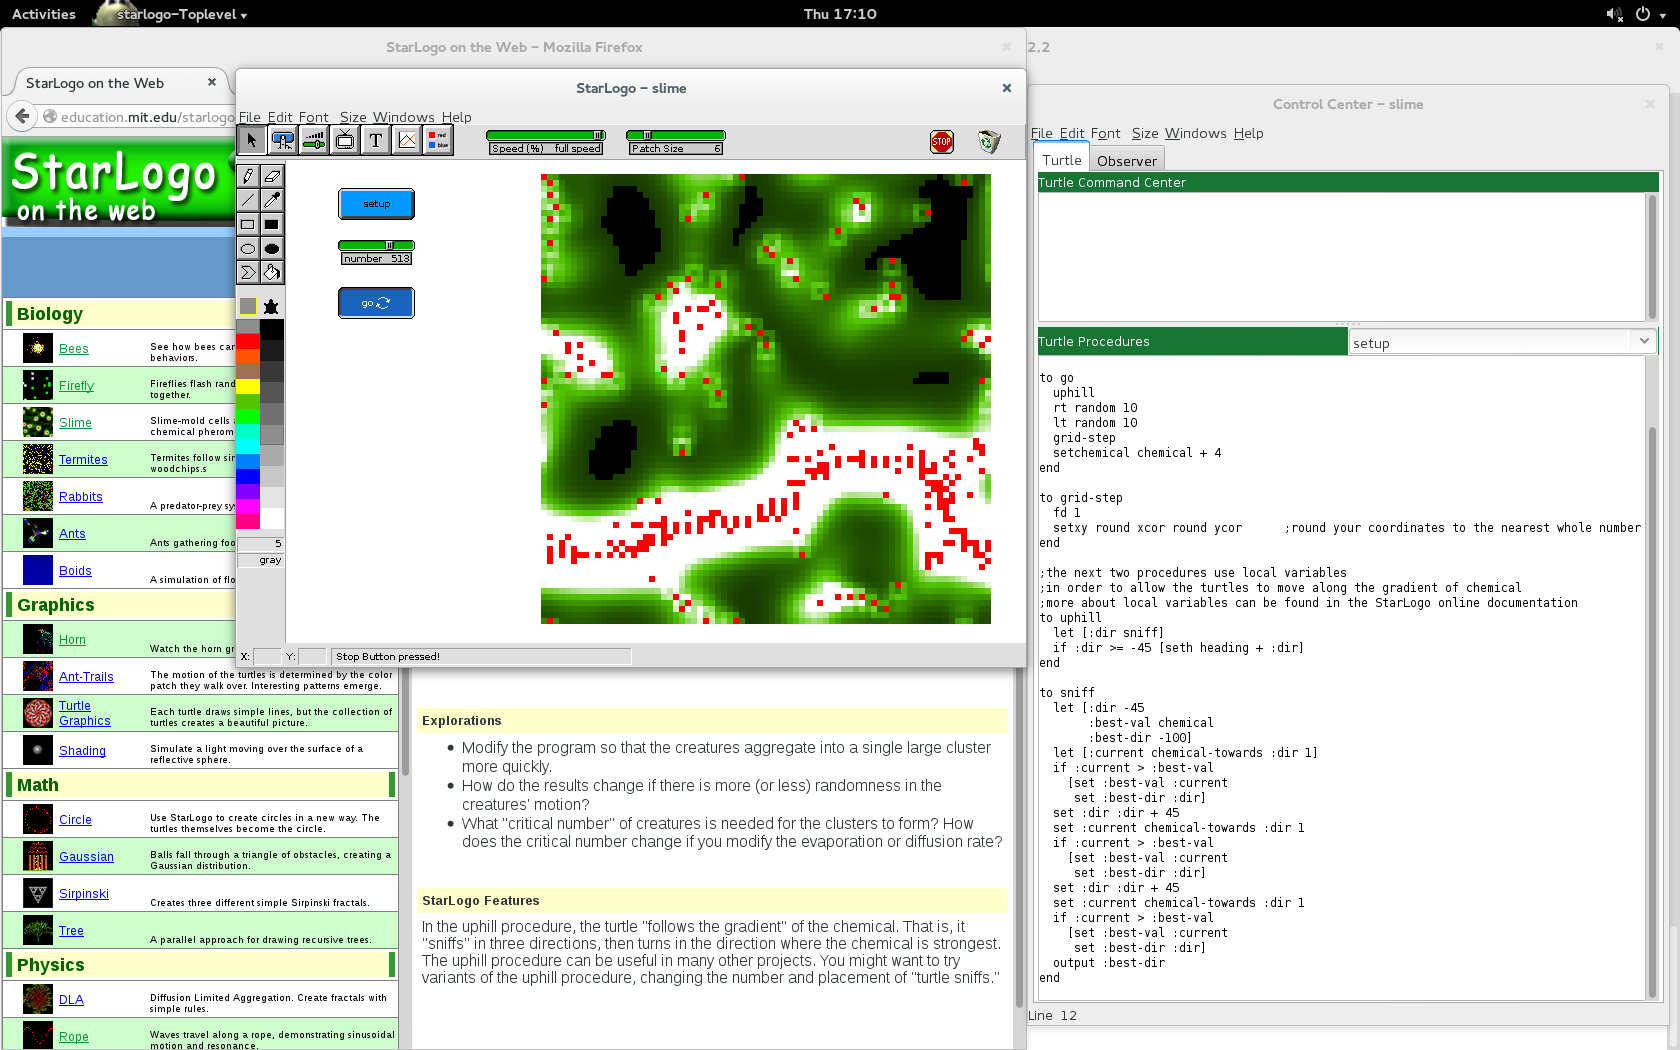
\includegraphics[width=\textwidth]{slimemold/mold10104-2.png}
	\end{center}
	\end{subfigure}
\hfill
	\begin{subfigure}[tbh]{0.30\textwidth}
	\begin{center}
	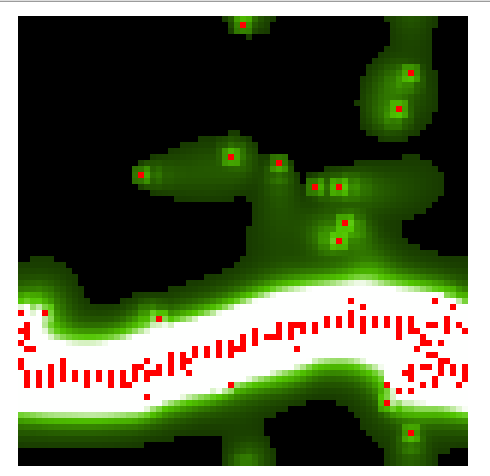
\includegraphics[width=\textwidth]{slimemold/mold10104-3.png}
	\end{center}
	\end{subfigure}
\caption{ Slime Mold with $x=10$ and $y=10$}
\end{center}
\end{figure} \label{mold1010}

%2020
\begin{figure}[tbh]
\begin{center}
	\begin{subfigure}[tbh]{0.30\textwidth}
	\begin{center}
	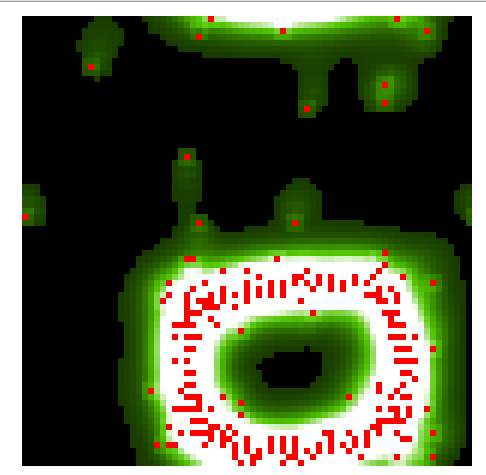
\includegraphics[width=\textwidth]{slimemold/mold20202-1.png}
	\end{center}
	\end{subfigure}
\hfill
	\begin{subfigure}[tbh]{0.30\textwidth}
	\begin{center}
	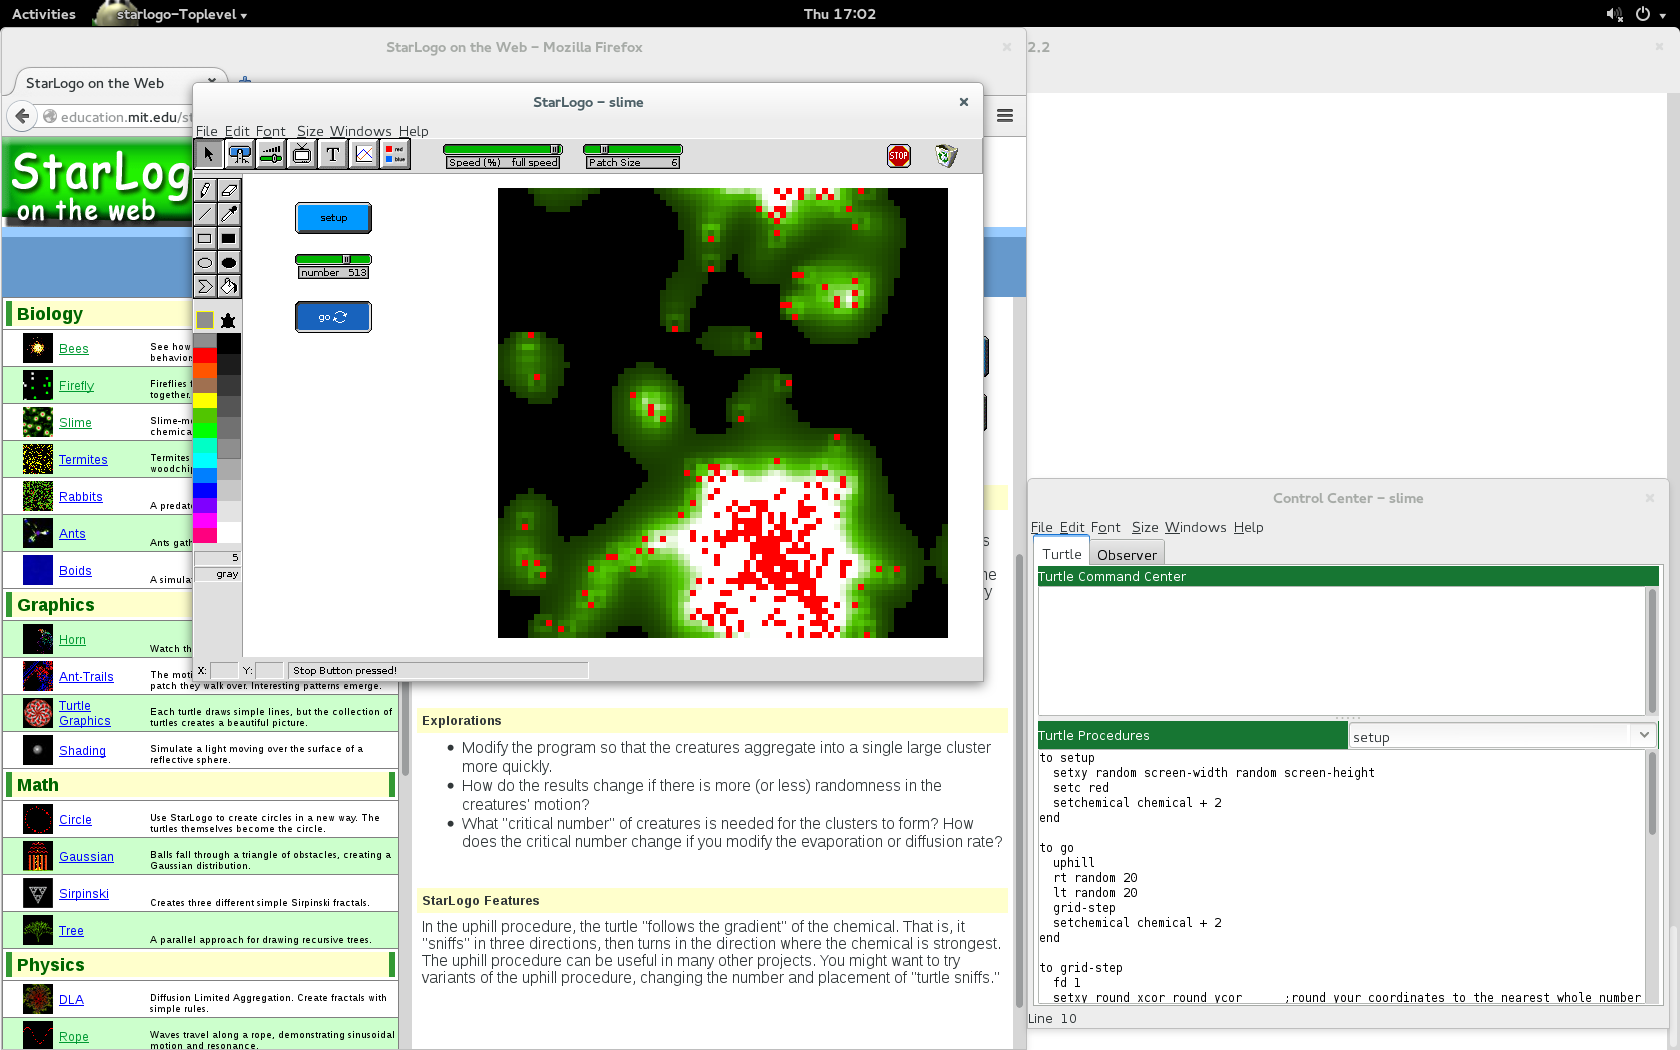
\includegraphics[width=\textwidth]{slimemold/mold20202-2.png}
	\end{center}
	\end{subfigure}
\hfill
	\begin{subfigure}[tbh]{0.30\textwidth}
	\begin{center}
	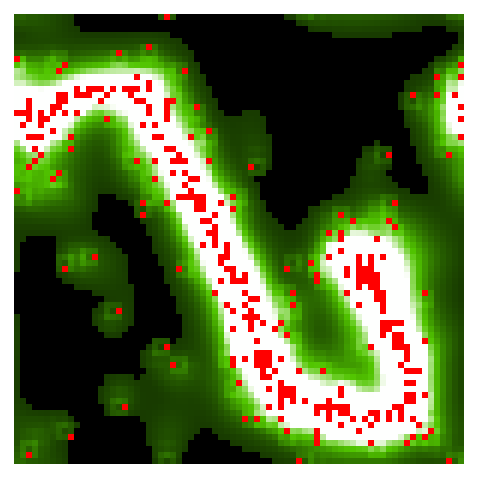
\includegraphics[width=\textwidth]{slimemold/mold20202-3.png}
	\end{center}
	\end{subfigure}
\caption{ Slime Mold with $x=20$ and $y=20$}
\end{center}
\end{figure} \label{mold2020}

%3030
\begin{figure}[tbh]
\begin{center}
	\begin{subfigure}[tbh]{0.30\textwidth}
	\begin{center}
	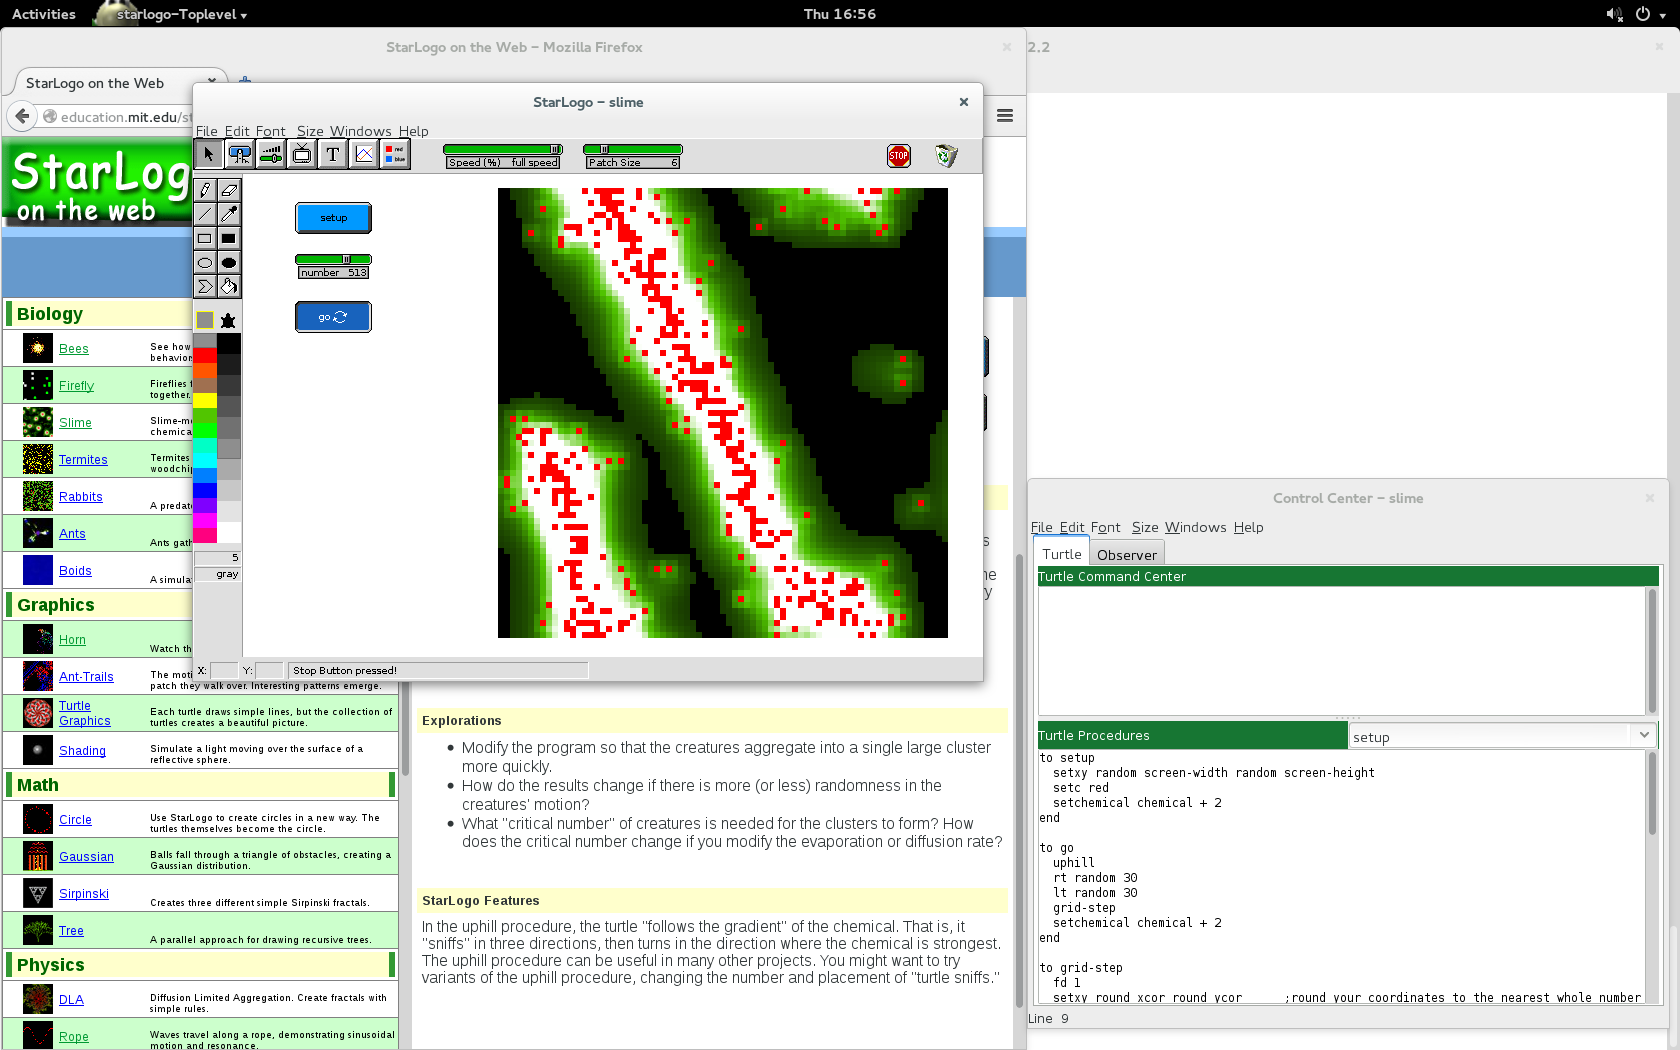
\includegraphics[width=\textwidth]{slimemold/mold30302-1.png}
	\end{center}
	\end{subfigure}
\hfill
	\begin{subfigure}[tbh]{0.30\textwidth}
	\begin{center}
	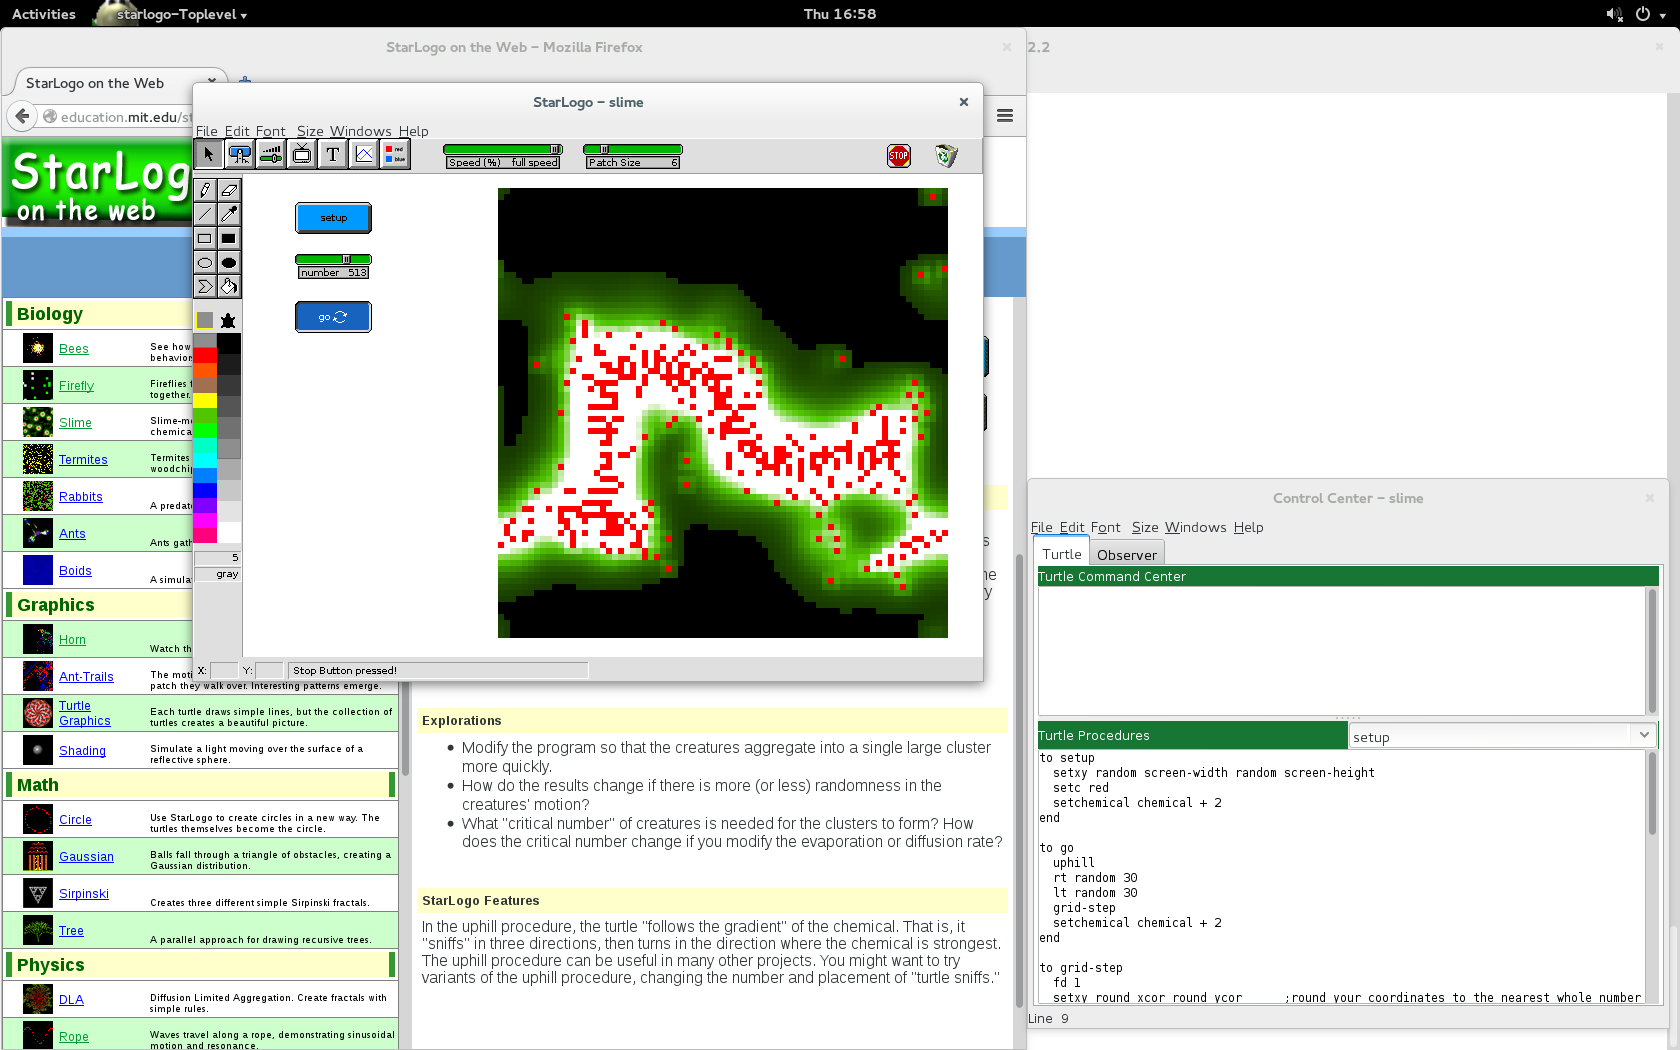
\includegraphics[width=\textwidth]{slimemold/mold30302-2.png}
	\end{center}
	\end{subfigure}
\hfill
	\begin{subfigure}[tbh]{0.30\textwidth}
	\begin{center}
	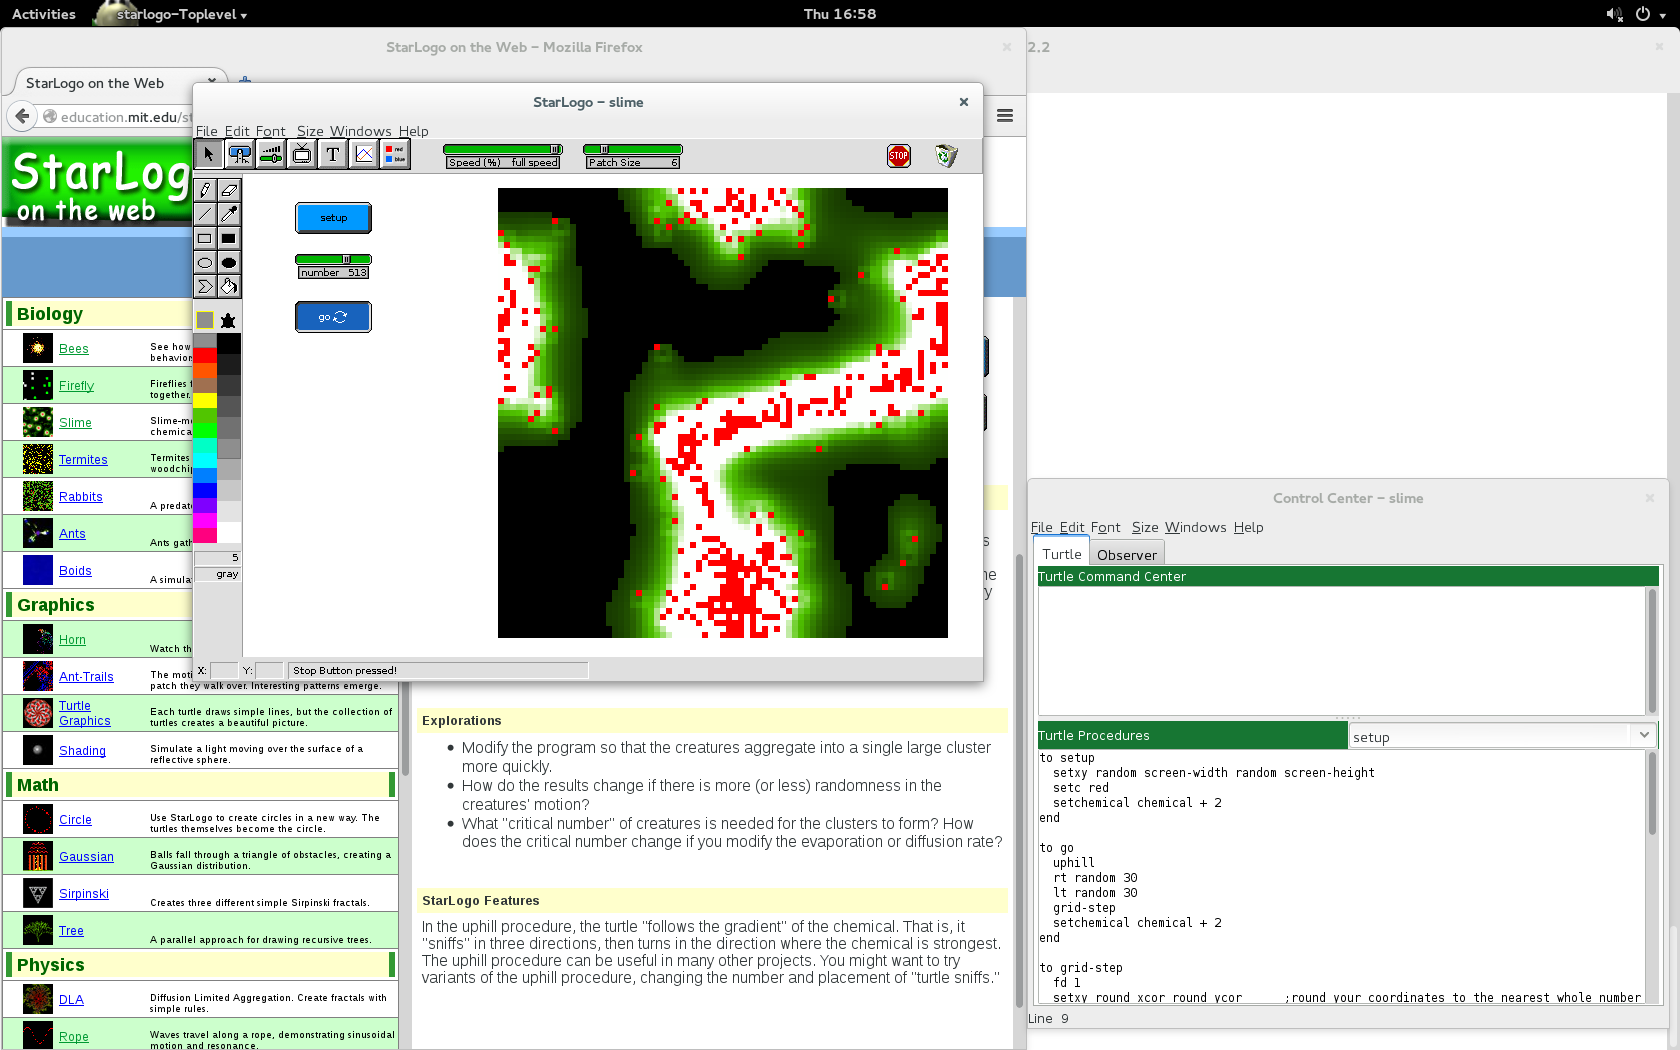
\includegraphics[width=\textwidth]{slimemold/mold30302-3diverge.png}
	\end{center}
	\end{subfigure}
\caption{ Slime Mold with $x=30$ and $y=30$}
\end{center}
\end{figure} \label{mold3030}

%7070

\begin{figure}[tbh]
\begin{center}
	\begin{subfigure}[tbh]{0.40\textwidth}
	\begin{center}
	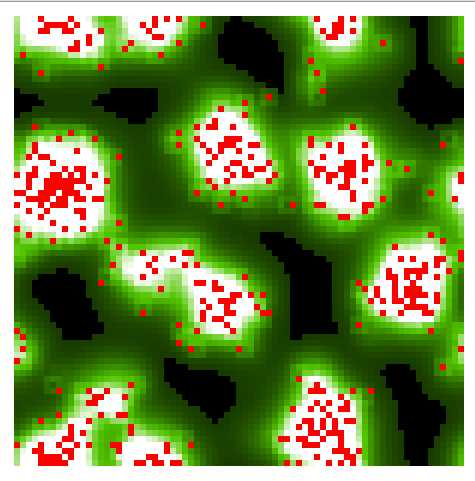
\includegraphics[width=\textwidth]{slimemold/mold70702-1.png}
	\end{center}
	\end{subfigure}
\hfill
	\begin{subfigure}[tbh]{0.40\textwidth}
	\begin{center}
	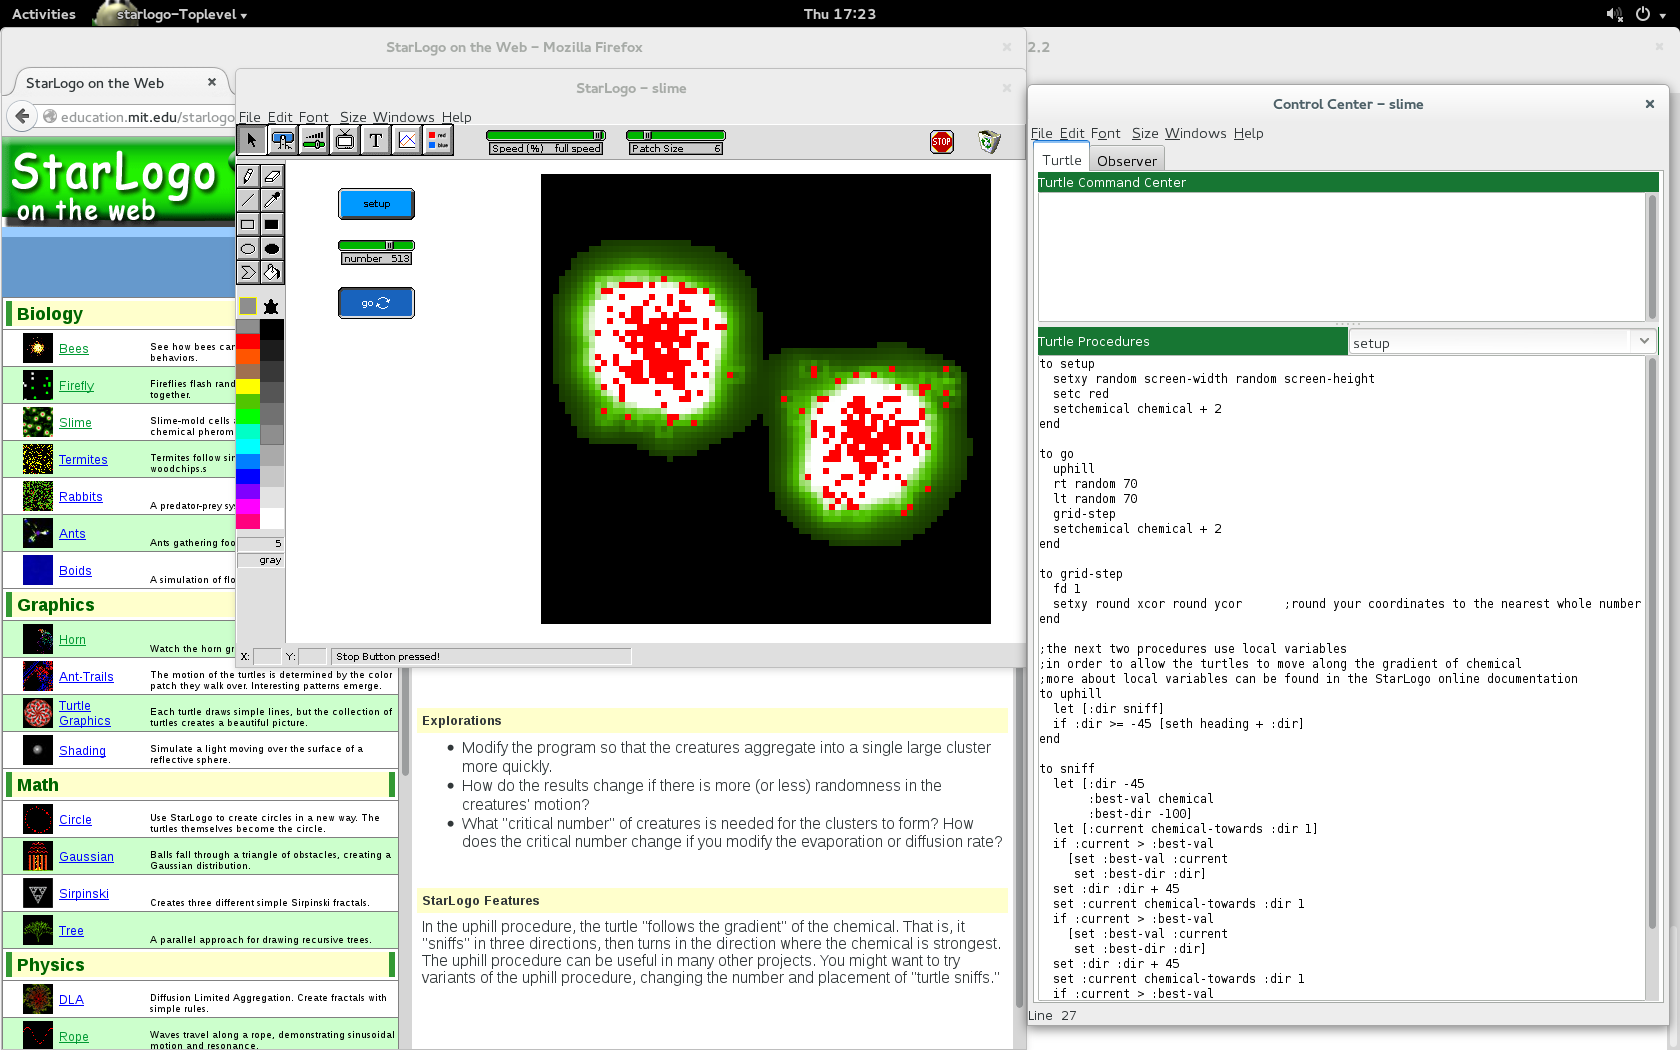
\includegraphics[width=\textwidth]{slimemold/mold70702-2.png}
	\end{center}
	\end{subfigure}
\caption{ Slime Mold with $x=70$ and $y=70$}
\end{center}
\end{figure} \label{mold7070}

\section{ Problem 4 }
\textbf{ Implement a bi-dimensional CA following the rules of ``The Game of Life.'' }\\
\newline
John Conway proposed a solitaire game called 'Life', currently known as 'The Game of Life'. He wanted to create a set of transition rules that were simple to write but also difficult to predict the outcome or overall behavior of the CA. The game had to meet the following criteria:

\begin{enumerate}
	\item There should not be any initial pattern for which there is a simple proof that the population can grow without limit.
	\item There should be initial patterns that apparently do grow without limit. Not all initial states should immediately yield trivial final states.
	\item There should be simple initial patterns that grow and change for a considerable period of time before coming to an end in three possible ways: fading away completely, settling into a stable configuration that remains unchanged thereafter, or entering an oscillating phase in which they repeat an endless cycle of two or more periods.
	\dots
\end{enumerate}

The rule set that Conway came up with is simple and uses the Moore neighborhood:
\begin{itemize}
    \item Birth: a previously dead cell comes alive if three neighbors are alive.
    \item Death: isolated living cells with no more than one live neighbor die; those with more than three neighbors die of overcrowding.
    \item Survival: living cells with two or three live neighbors survive.
	\dots
\end{itemize}

Using the above rule set and bi-directional grid, all of the criteria that Conway required appeared through running the Game of Life. There were oscillating phases and stable configurations that remained unchanged. A lot of the patterns died out or within a few generations turned into an stable configuration.

\begin{figure}[tbh]
\begin{center}
    \begin{subfigure}[tbh]{0.475\textwidth}
    \begin{center}
    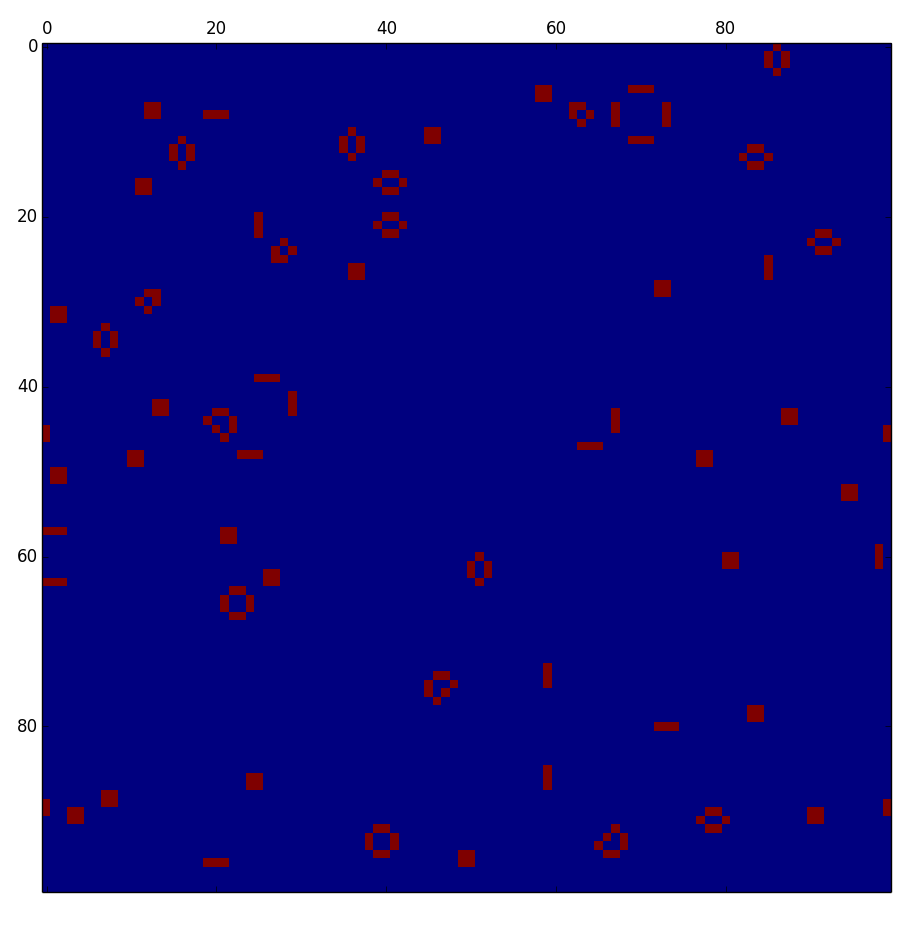
\includegraphics[width=\textwidth]{conway/game1.png}
    \caption{ Stabilized Game of Life with few oscillating phases }
    \end{center}
    \end{subfigure}
\hfill
    \begin{subfigure}[tbh]{0.475\textwidth}
    \begin{center}
    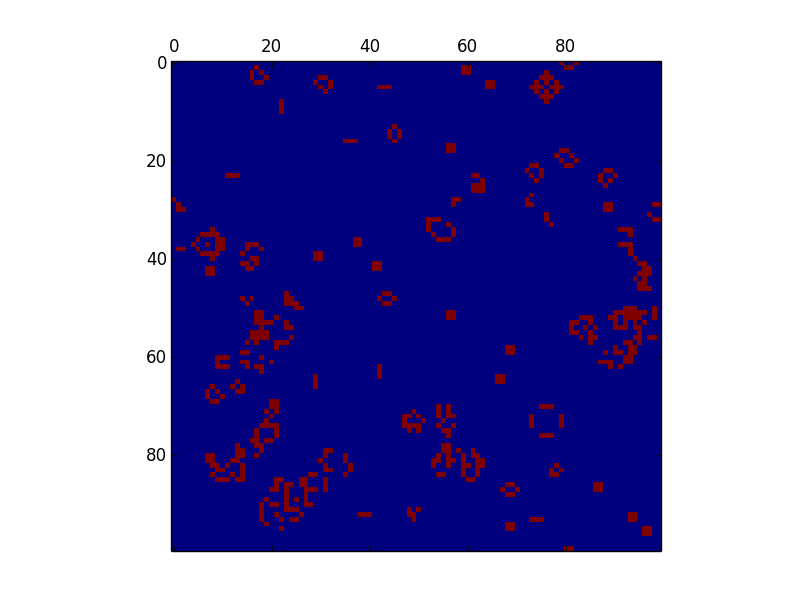
\includegraphics[width=\textwidth]{conway/game4.png}
    \caption{ Criteria 2 }
    \end{center}
    \end{subfigure}
\hfill
    \begin{subfigure}[tbh]{0.475\textwidth}
    \begin{center}
    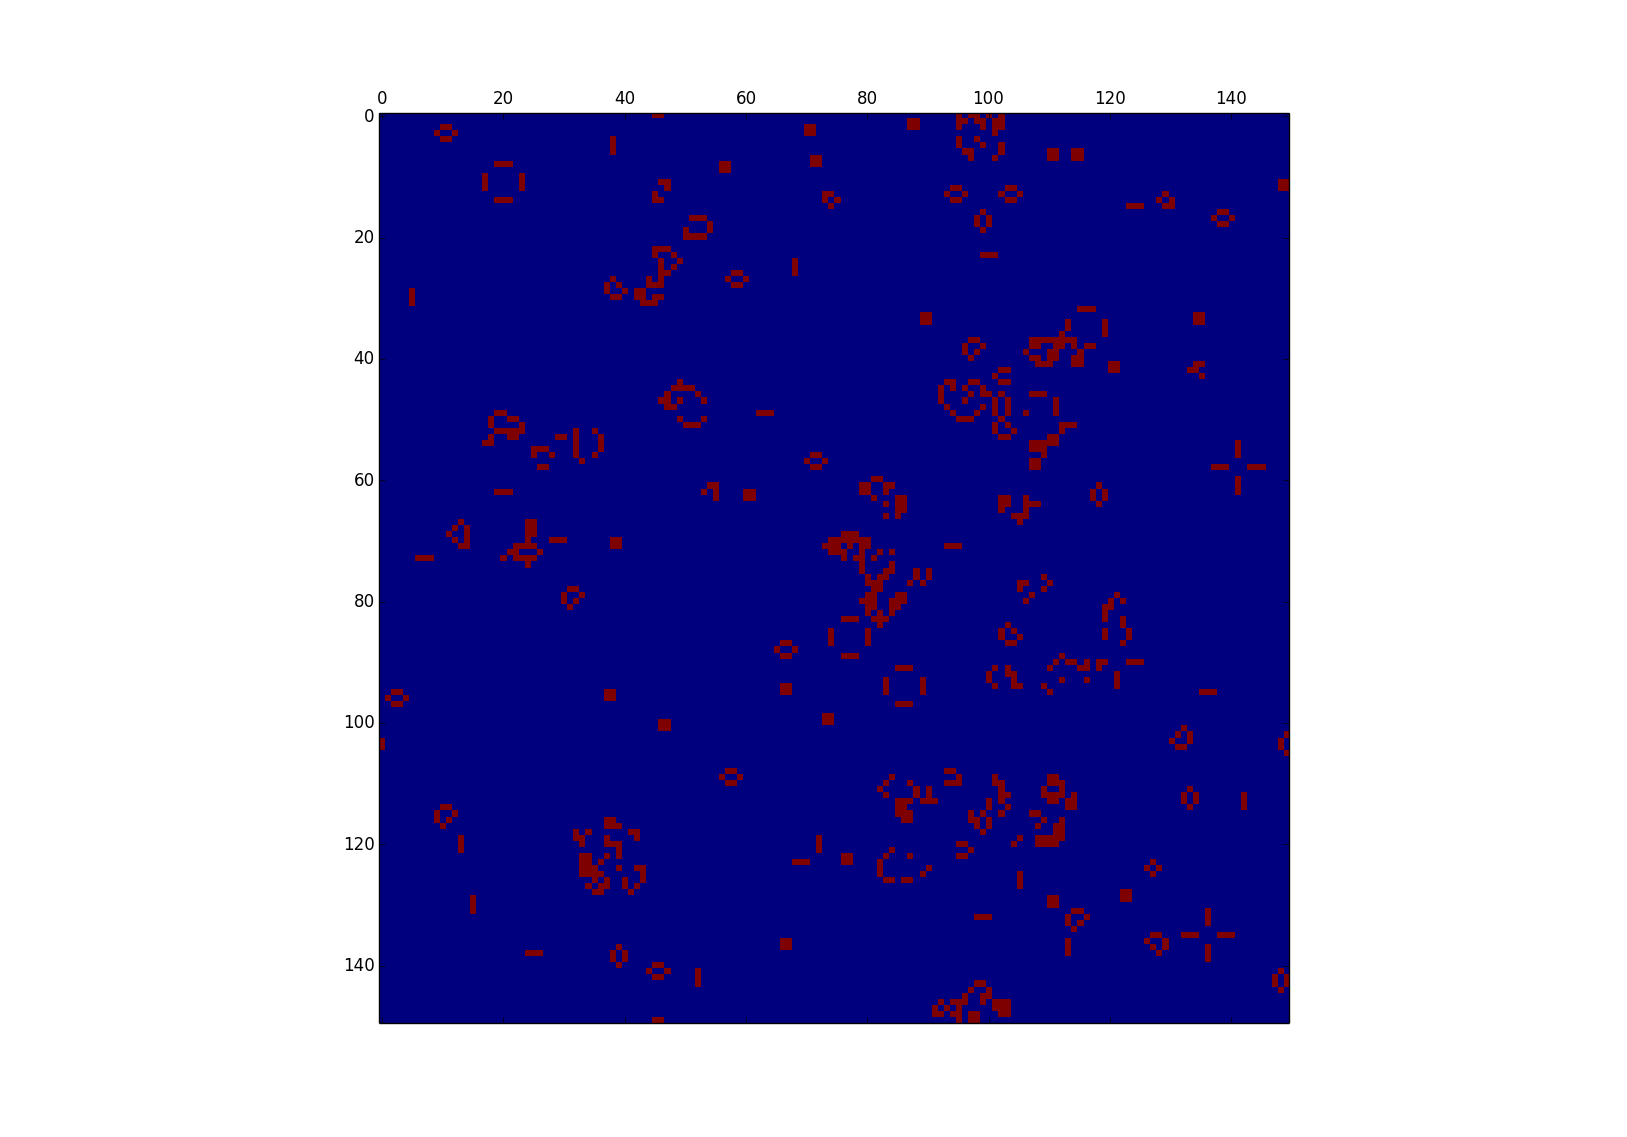
\includegraphics[width=\textwidth]{conway/game7.png}
    \caption{ Game in Progress }
    \end{center}
    \end{subfigure}
\hfill
    \begin{subfigure}[tbh]{0.475\textwidth}
    \begin{center}
    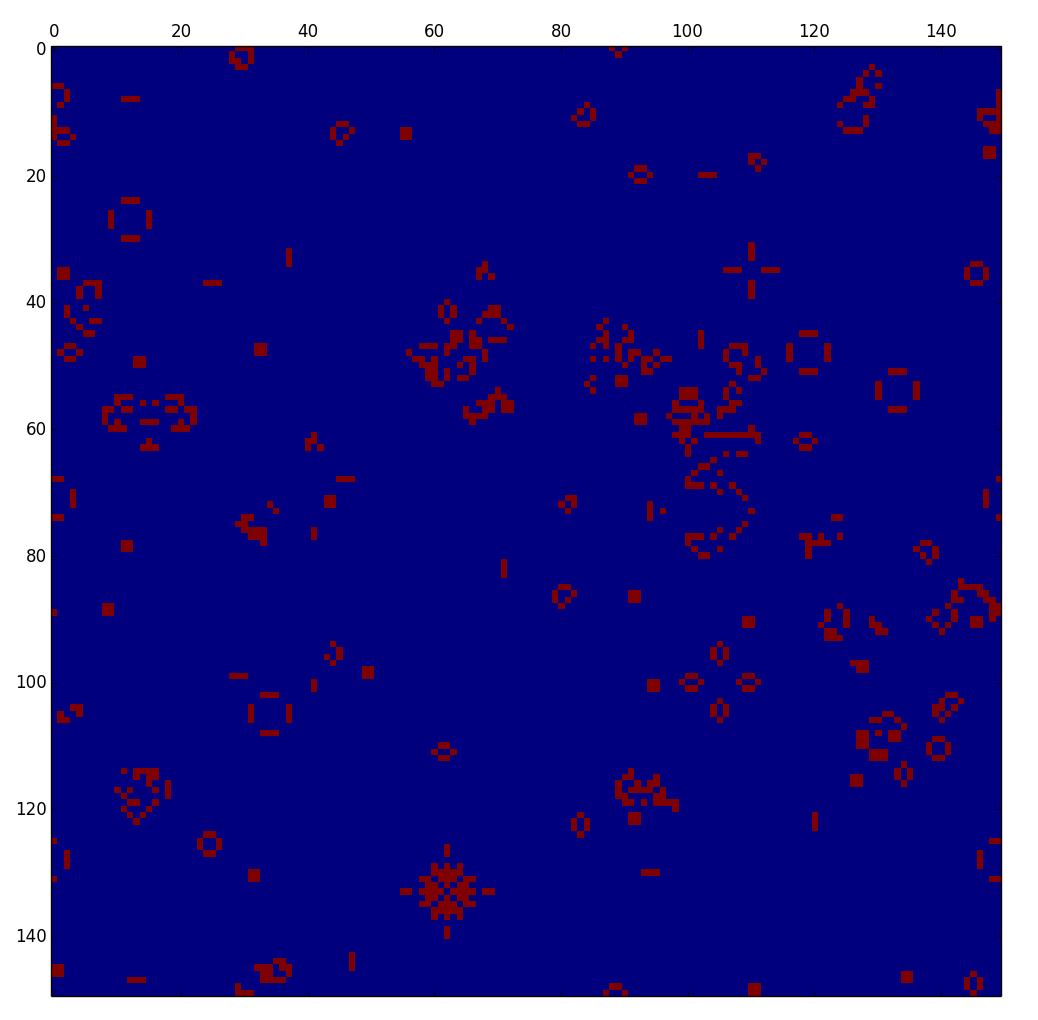
\includegraphics[width=\textwidth]{conway/game6.png}
    \caption{ Criteria 3 }
    \end{center}
    \end{subfigure}
\hfill
\end{center}
\caption{Plots of Various Games \label{conway} }
\end{figure}

% !TEX root = Simulation.tex

\chapter{DNA Computing - Text Chapter 9}


\section{ Problem 1 }
\textbf{ Name four problems that cannot be solved by a Turing machine. } \\
The Halting Problem, Mortality Problem, Busy Beaver Champion, and Rice's Theorem are four problems that cannot be solved by a Turing Machine. Undecidable problems is the type of problem that a Turing machaine cannot solve. These requre a yes/no answer, however, there isn't a possible computer program that will always give a right answer. It would sometimes give the wrong answer or run forever without giving an answer. Descriptions of algorithms taken from wikipedia.
\begin{itemize}
	\item The Halting Problem: Problem of determining, from a description of an arbitrary computer program and an input, whether the program will finish running or continue to run forever.
	\item Mortality Problem: Given a Turing machine, decide whether it halts when run on any configuration(Not necessarily a starting one).
	\item Busy Beaver Champion: A Turing machine that attains the maximum number of steps performed, or maximum number of nonblank symbols finally on the tape, among all Turing machines in a certain class. The Turing machines in this class must meet certain design specifications and are required to eventually halt after being started with a blank tape.It is undecidable by a general algorithm whether an arbitrary Turing machine is a busy beaver.
	\item Rice's Theorem:for any non-trivial property of partial functions, there is no general and effective method to decide whether an algorithm computes a partial function with that property.
\end{itemize}

\section{ Problem 2 }
\textbf{ Name four NP-complete and four NP-hard problems. } \\
The Traveling Salesmen Problem (TSP), Himiltonian Path Problem, Satisfiability Problem for Propositional Formulas or Propositions (SAT) Problem, and the Knapsack Problem are four NP-complete problems. The Halting Problem, Cook's Theorem, Maximum Clique Size (from3SAT), and Vertex Cover (from Independent Set).
\begin{itemize}
	\item TSP
\end{itemize}

\section{ Problem 5 }
\textbf{ The two most basic DNA sequencing techniques are known as a) Maxam-Gilbert and b) Sanger, after their proponents. Explain how each of these techniques work and contrast them. }\\
\newline
\textbf{Maxam-Gilbert}
The Maxam-Gilbert DNA sequencing technique was developed during 1976-1977. The first step is to radioactively label one end of the DNA fragment. Next, a chemical treatment is used to break a small sample of one or two of the four bases. The modification chemicals are controlled such that the concentration of them will introduce an average of one modification per DNA molecule. The modified DNA may then be cleaved by hot piperidine at the modified base. This labels the DNA fragments.\\
Next, the fragments of the reactions are separated based on size in a gel substance. Then the gel is exposed to an X-ray film to visualize the fragments. Dark bands on the film show the location of identical labeled molecules. \\
\newline
\textbf{Sanger}
The Sanger DNA sequencing technique was developed in 1977. It separates the two DNA strands and the strand to be sequenced is copied. However, the copied strand has chemically altered bases so that when a specified base is reached, it stops copying. The process is done for all four bases and then put back together like a puzzle to see the original piece of DNA.\\
\newline
Both techniques both use chemical reactions, however the Sanger technique requires the DNA to be cloned whereas the Maxam-Gilbert technique can use the raw DNA without prior modification to begin the sequencing. 


%%%  Done with chapters
% Bib stuff

\bibliographystyle{plain}
\bibliography{refs.bib}
\addcontentsline{toc}{chapter}{Bibliography}



% In our style file, appendices are numbered with capital letters
\appendix

\chapter{Supporting Materials}

Supporting ...

\chapter{Code}
Insert code here.   You can use the listing environment or use doxygen.



% chapters in backmatter don't have numbers, but they appear in the
% table of contents, and are numbered BM-X where X is the page number
% relative to where the backmatter begins.
% \backmatter


\end{document}
